%-----------------------------------------------------------------------------
%%	PACKAGES AND DOCUMENT CONFIGURATION
%-----------------------------------------------------------------------------

% Use `report` class with `USCthesis` package (style file) by Brian P. Gerkey
\documentclass{report}
% [options] can be any of these default/alternative flag:
%   dissertation/thesis, final/proposal, copyright/nocopyright,
%   fussy/sloppy, flushbottom/raggedbottom, clref/opref.
\usepackage[final]{USCthesis}

% Packages required by `USCthesis.sty`.
\usepackage{setspace}
\usepackage{tabularx}
% Filler text for formatting. Comment these lines out for real writing.
%\usepackage[english]{babel}
%\usepackage{blindtext}

% Other packages
% math
\usepackage{amsmath}
\usepackage{amssymb}
\usepackage{bm}
%% SI units
\usepackage{siunitx}
% graphic
\usepackage{graphicx}
\graphicspath{ {figures/}}
% bookmarks
\usepackage{navigator}
% indentation
\usepackage{indentfirst}
% table
\usepackage{dcolumn}
\usepackage{multirow}

\begin{document}

%-----------------------------------------------------------------------------
%%	TITLE PAGE
%-----------------------------------------------------------------------------

% Volume name could be added as option, e.g. `[Volume I]`.
\title{A Computational and Behavioral Analysis of Upper Extremity Movement of Non-Disabled and Post-Stroke Individuals}

\author{Chunji Wang}

% Committee list is only shown in `proposal` layout.
\committee{S.~Schaal & (Chair)\\*
           N.~Schweighofer\\*
           J.~Gordon & (Outside Member)}

% Submission information is only shown in `final` layout.
\majorfield{Neuroscience}
\submitdate{June 2017}

%-----------------------------------------------------------------------------
%%	PREFACE
%-----------------------------------------------------------------------------

% The preface environment prints the title page.
\begin{preface}

  % Dedication Page, which is truly unnecessary.
  \prefacesection{Dedication}
    This dissertation is dedicated
     \begin{quote}
         \raggedleft {\em To my friend Noman.}\\
     \end{quote}

  % Acknowledgement Page, which is also unnecessary for proposals.
  \prefacesection{Acknowledgements}
    % Better to separate LaTeX structure and content
    To my mother Yaxian and my father Jun, who have provided me love and emotional support with understanding and patience.

I would like to thank my advisor Professor Nicolas Schweighofer, who has provided guidance and swept away many blocks in the route of research. 
Also to my committee member Professor James Gordon and Professor Stefan Schaal, who evaluated my work with a critical eye and always gave valuable comments and feedback. 
Also to Professor Finley and Professor Liew who, together with all other members of Computational Motor Control and Learning Journal Club, provided a friendly environment for discussion.

Thanks to all my labmates: Yupeng, Sujin, Amar, Hyeshin, Youngmin, Victor and others in CNRL lab; BK, Irene, Andrew, Dorsa, Clarisa, Rini, Yuchen, Yi'an and others in MBNL lab; Chang, Natalia, Aram, Sungwoo and others in LCL lab.
Many cheerful (or tiresome) and fruitful discussions with them that brought insight to my work, and many small talks and chitchats in which we shared our gossips and complaints about our advisors and TA works.

Grateful to all program staff: Dawn Burke, Ariana Perez and Deanna Solorzano in NGP; Veronica Perez and Lydia Vazquez in BKN for their unfailing support and assistance.

Special thanks to my friend Zixuan, whose vibe and grit encourage me not to fall too behind;
To Tian Chen, who boosted my confidence at times of difficulties; 
To my friend Liu Chang, whose cheerfulness was highly infective.
To my friend Zhiqiang, Zhihui, Feng Ying and others in the Youth Group whose altruistic and cheerful characters remind me the world is still good.
Thanks to my fellow badminton players Wenjian and Tianjiao, together with whom I forget everything in the world enjoying the sport.
And to all my friends these years along the way who listened to my boring problems and provided support in many ways.





  \tableofcontents
  \listoftables
  \listoffigures

  % Abstract Page
  %\prefacesection{Abstract}
  %  \input{abstract.tex}
\end{preface}

%-----------------------------------------------------------------------------
%%	CONTENT STRUCTURE
%-----------------------------------------------------------------------------

% Better to separate LaTeX structure and content
\outline{1}{Introduction}
\chapter{Introduction}
\raggedbottom
\label{cha:introduction}


\section{Motivations}
\label{sec:motivations}
Human upper extremity movement is an essential component that is necessary for everyday life.
Many, if not all, activities cannot be completed without fluent upper extremity movement control.
Study of upper extremity movement sheds light on the interesting subject of how humans control the body to move around and perform certain tasks, and has attracted many researchers’ attention. 
As a major subset of upper extremity movement, the study of reaching movement is approached via many techniques including kinematics analysis \cite{Hogan2009}, optimal control \cite{Todorov2002}, synergy analysis \cite{Bockemuehl2010}, uncontrolled manifold \cite{Domkin2005} etc. 
The study of rehabilitation and recovery of reaching movement of post-stroke individuals, in parallel with studies of healthy subjects, also provides valuable insights about the cause of pathological movement and recovery mechanisms, and can help understand the pattern and structure of recovery hence facilitate it \cite{Liebermann2012}.

\section{Motor Control of Reaching Movement}
Humans quickly choose a movement duration for a reaching movement, and the decision usually works very well with the specific goal and the context \cite{Tanaka2006}. 
This decision of movement duration, or of any movement, is poorly understood. 
The first prominent work on this topic was by Fitts whose work was referred as “Fitts’ law” \cite{Fitts1954}, which formulized the relationship between movement duration and task difficulty. 
Works by R. Schmidt in 1980s \cite{Urbin2011} focused on ballistic movement, and reached to the conclusion that, movement variability was smaller at longer movement, when the movement duration was in the range from 100 to 200 milliseconds. 
However, none of these studies gave theory of how and why a certain movement duration is determined. 
There are several competing theories about how the duration of a movement is determined. 
One of the hypotheses is “time discounting” of reward, based on the idea that reward in the future is discounted comparing an immediate reward \cite{Shadmehr2010}.
Although this hypothesis has its base on physiological studies \cite{Johnson2002}, but the discounting time constant is in the range of days or months, much longer than the time scale of reaching movement, which is in seconds. 
Whether discounting works within seconds remains to be confirmed. 

To understand the decision process therefore appears to be an interesting question. 
This work propose an alternative mechanism by looking at endpoint variance induced by two kinds of motor noise: constant noise (CN) and signal dependent noise (SDN).
We show strong evidence that effort, together with CN and SDN, determined movement duration.

In the first two chapters of this thesis, I investigate how the duration might be determined, how this decision process can be traced through the endpoint variability of reaching movement. I then demonstrate this decision process through an stochastic optimal control model. 
In Chapter \ref{cha:movementtime}, I present an experiment looking at how endpoint distributions depend on the duration of movement. 
In this experiment, we investigate the relationship between endpoint variability and movement duration, as well as the movement duration that is chosen by subjects.
In Chapter \ref{cha:optimalcontrol}, I present the development of a stochastic, open-loop optimal control model that demonstrate a possible mechanism of how movement variability, together with effort, determines movement duration.

The significance of this work is threefold. First, we re-estimated the levels of CN and SDN in reaching movements using optimal control model. 
CN and SDN have been estimated in several works about saccadic \cite{VanBeers2007} and reaching movements \cite{VanBeers2004}, but our result yields better fit with data, and requires no extra noise parameters comparing with \cite{VanBeers2004}. 
Second, we show that in reaching movement, there exists an intermediate movement duration that minimizes endpoint variance. 
This gains our understanding of the relationship between movement duration and variability, and serves as an extension to the famous Fitts’ law \cite{Fitts1954} and similar studies on saccadic movement \cite{VanBeers2007}. 
This work also extends the impulse variability theory \cite{Urbin2011} to longer movement duration. 
Third, by showing that subjects chose durations of reaching movements that are longer than those minimizing endpoint variance, we gave a clear evidence that effort plays a role to determine movement duration in reaching movements.


\section{Recovery of Kinematics Performance}
The same reaching task may have different ways to perform, since the degrees of freedom of the arm may be larger than that of the task. 
For example, the trajectory from home to target can be straight or curved. 
Even the same trajectory can be achieved with different joint coordination patterns, from different populations, i.e. healthy subjects and post-stroke individuals \cite{Cirstea2000}. 
This is important because the efficiency of different patterns of joint coordination can be different, and therefore can be correlated with performance \cite{Sibindi2013}. 
In this project, we look at joint coordination patterns during a vertical pointing task, in both healthy and post-stroke individuals, and its relevance to movement performance.

A lot of work \cite{Dipietro2009} focus on motor learning and recovery in hand space, which is usually the space of planned activity and experiment design. 
However, motor learning and recovery can also be investigated in joint space, which involves coordination of different joint angles. 
Because the dimension of hand space or task space is often smaller than the degree of freedom of joint space, the same hand position, orientation and velocity can be achieved by different combinations of joint angles. 
Thus, the improvements of performance in hand space can due to either compensatory movement or true recovery \cite{Cirstea2000, Levin2002, Shaikh2014} of normal movement patterns.
The notion of compensatory mechanism and true recovery can be confusing \cite{Levin2009}. 
Here we do not consider recovery in a neural level, but rather the performance level \cite{Levin2009}, which is essentially in the language of kinematics and dynamics. 
For example, one common compensatory movement during reaching forward movement is trunk movement. 
Levin and colleague have many works investigating how trunk and shoulder movements serve as compensatory mechanism for severe impaired individuals \cite{Cirstea2000}. 
It is shown that with compensatory movement of the trunk, the performance in hand space is worse than that without. 
However, even though the trunk is constrained and does not contributes any compensatory movements, the arm by itself can have compensatory movements. 
How the performance of a reaching movement in hand space is related to compensatory movements of the arm is still unclear. 
A better understanding on this topic can help clinical practice to plan a rehabilitation strategy to maximize performance.

In Chapter \ref{cha:armeospring}, I looked into joint coordination patterns of both healthy subjects and post-stroke individuals, with kinematics data at both endpoint and joint space. 
We used Principal Component Analysis (PCA) to measure motor synergies.
We also looked at redundancy exploitation in the reaching movements \cite{Singh2016}.

\section{Dynamic Mixed Effect Model of Stroke Rehabilitation}
Observational rehabilitation studies are important as they shed light on effective factors in rehabilitation.
Among the multi-variate techniques used to analyze data from these studies are regression models, including mixed effect models that account for individual variations. 
Regression models have been used to predict stroke recovery \cite{Johnston2000} and response to interventions \cite{Stinear2006}.
Such models exhibit room for improvement because they are based on aggregate clinical scales, but also, we hypothesize, because they do not model the time-varying processes of recovery. 
In contrast, dynamical models naturally encode time in differential equations that model “changes in states”. 

State Space Model (SSM) is a dynamic model that describes a dynamic process via state vectors in state space.
The field of motor adaptation and learning constantly uses SSM to model motor learning and adaptation data.
Unlike regression models, state-space models can describe processes that respond, simultaneously or with a latency, to time-varying inputs or stimuli.
This approach will allow us to test for causal relationships between training, learning, and recovery. 
In addition, the model will allow us to obtain a detailed time course of time window of plasticity. 
Although never applied to stroke recovery, such models have been applied successful to model the action of drugs on a range of diseases \cite{Tan2000}.

One of the challenges of using SSM is to incorporate random effects into SSM, which is computationally not trivial and offered by few statistics toolboxes.
Random effects in SSM is desirable especially in observational rehabilitation studies because of the high variability in stroke rehabilitation.
In Chapter \ref{cha:dose}, we show that under certain conditions, state space equation is equivalent to differential equation, and therefore share the same solution, which is a nonlinear function.
We then use nonlinear mixed effect model to estimate the parameters in this nonlinear solution.


% Research Project 1
\outline{1}{The Duration of Reaching Movement is Longer than Predicted by Minimum Variance}
\chapter{The Duration of Reaching Movement is Longer than Predicted by Minimum Variance}
\label{cha:md}


\section{Abstract}
Whether the central nervous system minimizes variability or effort in planning arm movements can be tested by measuring the preferred movement duration and endpoint variability. Here we conducted an experiment in which subjects performed arm reaching movements without visual feedback in fast-, medium-, slow-, and preferred-duration conditions. Results show that 1) total endpoint variance was smallest in the medium- duration condition and 2) subjects preferred to carry out movements that were slower than this medium-duration condition. A parsimonious explanation for the overall pattern of endpoint errors across fast, medium, preferred, and slow movement durations is that movements are planned to minimize effort as well as endpoint error due to both signal-dependent and constant noise.

This work was published at \textit{Journal of Neurophysiology} on August 24th, 2016, collaborators are Yupeng Xiao\footnote{\textit{Neuroscience Graduate Program, University of Southern California, Los Angeles, California}}, Etienne Burdet\footnote{\textit{Bioengineering Department,Imperial College, London, United Kingdom}}, James Gordon\footnote{\label{bknpt}\textit{Biokinesiology and Physical Therapy, University of Southern California, Los Angeles, California}}, and Nicolas Schweighofer\footnotemark[\ref{bknpt}]. Nicolas Schweighofer is the corresponding author. Yupeng Xiao shares the first authorship with Chunji Wang, the writer of this thesis. This chapter reprints the original published paper with permission from Chunji Wang and Nicolas Schweighofer.

\section{Introduction}

Although most motor tasks can be carried out in an infinite number of ways with our redundant musculoskeletal system, arm movements exhibit striking regularities. 
In particular, the durations of reaching movements vary systematically with the amplitudes and the directions of movements \cite{Gordon1994}. 
According to the optimal control theory of human motor control (e.g., \cite{Flash1985, Hoff1994, Uno1989}), these regularities correspond to the minimum of a cost function that the central nervous system (CNS) considers in planning motion. Despite much research on this topic, however, it is still unclear how the CNS determines the duration of movement during planning. The stochastic optimal control model of Harris and Wolpert (1998, 2006) proposes that the CNS determines movement planning by minimizing the movement endpoint variability due to signal-dependent noise. Although this model successfully predicts trajectories and durations of saccadic eye movements and planar arm reaching movements, it is not clear whether movement endpoint variability or effort is minimized. Indeed, mathematically, the expression of movement endpoint error due to signal-dependent noise in the motor commands and the expression of effort are equivalent \cite{OSullivan2009}.

Minimizing effort (or, equivalently, minimizing endpoint variability due to signal-dependent noise) will slow down planar movements, because the torques necessary to move the arm decrease with an increase in movement duration\footnote{The rigid body dynamics $\tau = M(q)\ddot{q} + C(q,\dot{q})\dot{q}$, where $M$ is the inertia matrix and $C$ represents the Coriolis and centrifugal forces and is a quadratic function of the velocity. As the velocity decreases linearly with movement duration and the acceleration decreases quadratically, the torques required to move the arm decrease in a quadratic fashion with an increase in movement duration. Assuming that effort is, e.g., a quadratic or linear function of these torques, this implies that the effort will decrease at least cubically \cite{Shadmehr2016} with a linear increase of the movement duration.}. 
For instance, movements performed by the right hand to leftward targets are slower than movements to rightward targets \cite{Gordon1994,Park2016}. This can be attributed to greater effort (or equivalently signal-dependent noise) for leftward targets because of greater inertia at the hand for these movements \cite{Cos2011, Guigon2007, Schweighofer2015}. 

In addition to signal-dependent noise, motor commands are also corrupted by constant noise \cite{VanBeers2007, VanBeers2004}. Although such constant noise was not considered in the models of \cite{Harris1998, Harris2006} and of \cite{OSullivan2009}, it can be quite substantial. For instance, by fitting the endpoint distributions generated by simulated arm movements to actual data, van Beers et al. \cite{VanBeers2004} estimated that the standard deviation of constant noise is about twice that of signal-dependent noise. 
Minimizing variability due to constant noise shortens the movement, because variability due to this type of noise increases with movement duration (see Fig. 1 in \cite{Todorov2005} for simulation results of the respective effects of signal-dependent and constant noise for varying durations of arm movements). 
Thus minimizing variability due to both signal-dependent and constant noise would yield a minimum that could determine movement duration. 
Correspondingly, our first hypothesis is that the CNS chooses intermediate reaching movement durations to minimize endpoint variability in the face of signal-dependent and constant noise.

While minimizing endpoint variability due to both signal-dependent and constant motor noise would be sufficient to determine the duration of movements, the results of \cite{Burdet2001}  suggest that effort minimization contributes to movement planning in addition to noise. 
In that experiment, training arm reaching movements in a divergent force field led to reduced endpoint variability by increasing cocontraction of antagonist muscles. If the CNS only minimized endpoint variability, then it would use this energetically costly cocontraction strategy to reduce endpoint error \cite{Osu2004}. The fact that habitual movements (performed without force field) yield more relaxed muscle activity than in the experiment of \cite{Burdet2001} suggests that the CNS also minimizes effort. 
Minimization of effort independently from minimization of endpoint variability due to signal-dependent and constant noise sources would lengthen movement duration.

Our second hypothesis is therefore that the CNS chooses intermediate durations that are longer than those minimizing variability. 
To test these two hypotheses and examine how humans select movement durations, we conducted an arm movement experiment without visual feedback and measured endpoint variability in movements of four duration conditions, fast, medium, slow, and preferred, in which subjects choose to move at their preferred speed. The results verify our hypotheses, providing evidence for the concurrent minimization of effort and variability due to signal-dependent and constant motor noise.

\section{Methods}
Eleven young adult right-handed volunteers (between 20 and 30 years old; 3 women, 8 men) with no declared neurological impairments gave written informed consent to participate in the experiment described below, approved by the University of Southern California Ethics Committee.

Subjects performed reaching movements with their right arms to one of two targets at \ang{45} and \ang{135} (relative to the rightward direction parallel to the body) without online visual feedback in four conditions: preferred, fast, medium, and slow (Figure \ref{fig:mt-experiment}, A and C).  
Hand movements were recorded via a digital pen moving on a tablet (Wacom Tech). 
The tablet height was positioned such that the arm was moving approximately in a two-dimensional horizontal plane, with movements primarily involving horizontal shoulder and elbow rotations. 
The home position was placed such that the shoulder formed approximately a \ang{45} angle with the coronal plane and the elbow angle at \ang{90}. 
The distance from home position to targets was 7.4 cm. 
Target directions (\ang{45} and \ang{135}) were selected to maximize the difference in inertia at the hand (see Gordon et al. 1994). 
To minimize fatigue due to the large number of trials, the forearm was supported with a sling attached to a $\sim$4-meter-long cable hanging from the ceiling. 
Because of the long cable length, the pendulum effect was small.

At the beginning of each trial, subjects saw the home position, the target, and the cursor presented on a computer screen facing the subjects. 
Subjects were instructed to keep the cursor within the home position, and to move toward the target after a “go” signal at which moment all visual feedback was cleared. 
Final cursor position was displayed for 1 second after the recording period (900 ms for fast, 1,400 ms for intermediate, 2,400 ms for preferred and slow movement conditions). 
In the preferred condition, subjects reached for the targets as accurately as possible using their own selected movement duration (they were instructed to “reach naturally”). 
In the fast, medium, and slow conditions, subjects reached for the targets quickly ($\sim$350 ms), at a medium speed (400--800 ms), and slowly ($\sim$1,200 ms), respectively (Figure \ref{fig:mt-experiment} B). 
When the movement duration was outside of the range, a “too fast” or “too slow” message was displayed and the trial was repeated.
 
\begin{figure}
	\centering
	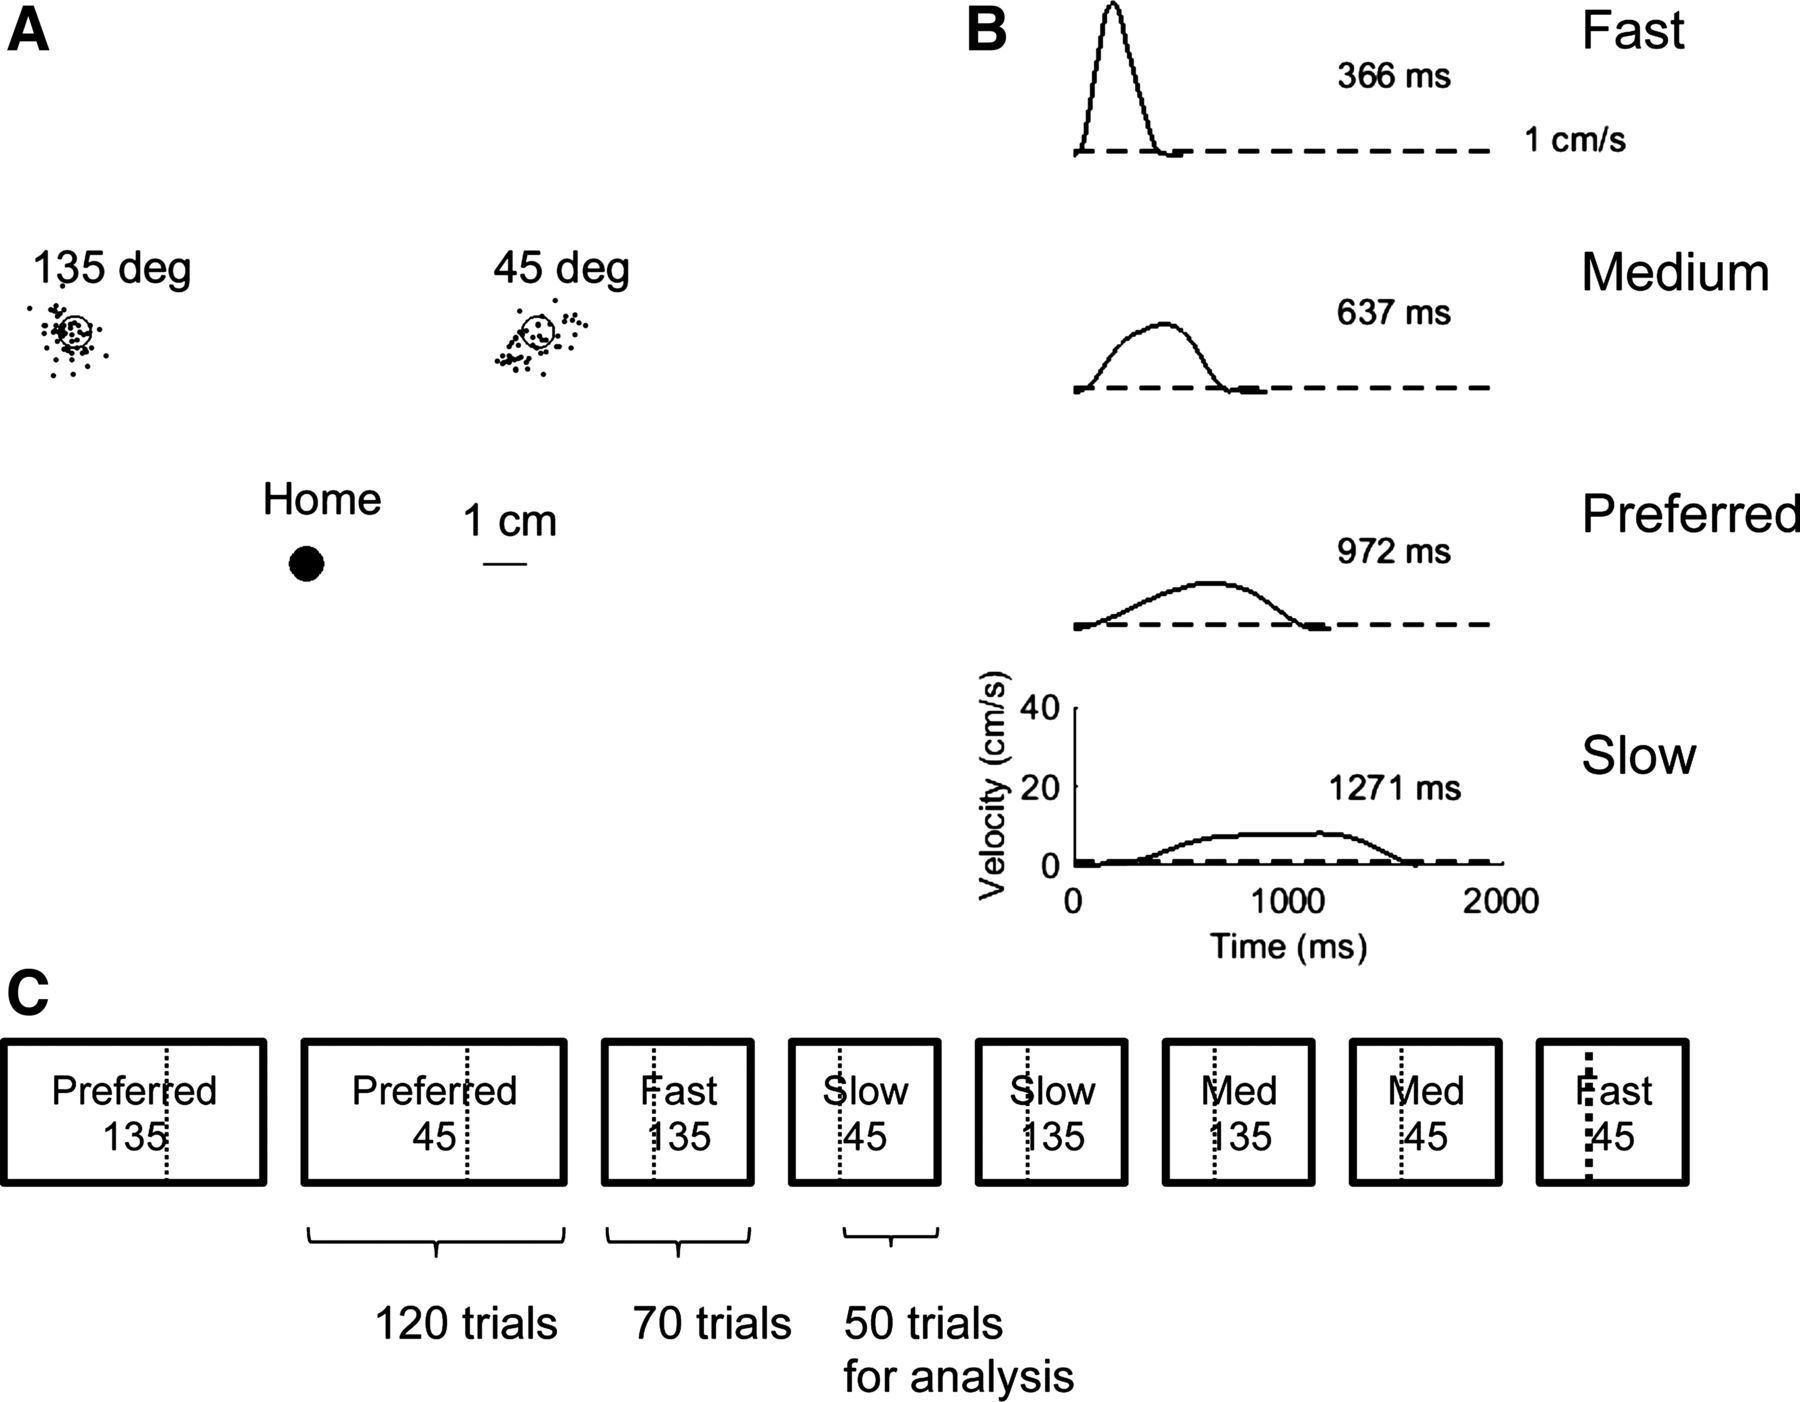
\includegraphics[width=0.8\linewidth]{figures/MT-experiment}
	\caption[Methods overview]{Methods overview. A: subjects performed horizontal reaching movements without online visual feedback to \ang{45} and \ang{135} targets in 4 duration conditions: preferred, fast, medium, and slow. The black dots around the targets show end points for 1 subject in the preferred condition. For each condition and each target, we measured endpoint variability from the variance of the endpoint distribution. B: example of velocity profiles in the 4 conditions: preferred, fast, medium, and slow. The movement duration was determined via a tangential velocity threshold of 1 cm/s. C: timeline of the experiment: example of the schedule for 1 subject. The 2 preferred movement blocks were always given first to avoid biasing the preferred duration by other conditions (the order of the 2 blocks were counterbalanced across subjects). The other 6 blocks (3 conditions, 2 targets) were then given, with the order counterbalanced for targets and conditions. Only the last 50 trials of each block (shown by dotted line) were analyzed, to remove possible initial drift and carryover in movement duration at the beginning of the blocks.}
	\label{fig:mt-experiment}
\end{figure}

Subjects first practiced all conditions in a familiarization session with online visual feedback of the cursor position, with 25 trials in each condition. 
To avoid possible carryover effects, the preferred movement duration condition was performed first, with the order of the two targets counterbalanced across subjects (Figure \ref{fig:mt-experiment} C). 
Subjects performed 120 trials for each target in the preferred condition and then 80 trials in the other six conditions (3 movement durations, fast, medium, slow for both targets), which were counterbalanced across subjects. 
The numbers of trials were determined in a pilot study, in which we noted that movement duration and final error stabilized only after a few dozen trials and that more trials were needed in the preferred condition for this stabilization to occur. 
This was confirmed in preliminary mixed-model analysis of the actual experiment, which showed a significant effect of a trial covariate on movement duration when all trials were considered. This effect disappeared (P $>$ 0.05) when only the last 50 trials in each condition and target were analyzed. Thus, for each subject, 400 movements were analyzed (50-trial block for each target in the 4 duration conditions).

Endpoint variance was computed by the trace of the covariance matrix of the endpoint distribution (Figure \ref{fig:mt-experiment} A). Because total endpoint variance was highly right-skewed, we analyzed the natural logarithm of total variance, which was approximately normal, as shown by both absolute values of skewness and kurtosis $<$ 2. Movement duration (MD) was computed with a velocity threshold of 1 cm/s across all conditions (Figure \ref{fig:mt-experiment} B).

We report the estimates of fixed effect parameters. MD and mean logarithm of variance were analyzed with mixed-effect models, with condition (fast, medium, preferred, and slow) and target (\ang{45} and \ang{135}) and their interaction as fixed effects and subjects as random intercepts. Bonferroni corrections were used for multiple comparisons. We used SPSS 18 with Restricted Maximum Likelihood method for these statistical analyses.

\section{Results}

Mixed-model analysis shows significant fixed effects of condition and target on MD (both with P $<$ 0.0001) as well as a significant condition $\times$ target interaction (P $<$ 0.0001; Figure \ref{fig:mt-data} A). Overall, the subjects’ preferred MDs were longer than the medium MD and shorter than the slow MD (Figure \ref{fig:mt-data} A; P $<$ 0.0001). In addition, MD was overall smaller for targets at \ang{45} compared with targets at \ang{135} (Figure \ref{fig:mt-data} A). Individual comparisons with Bonferroni corrections show that MD was shorter for the target at \ang{45} compared with the target at \ang{135} for the fast condition (P = 0.003), the slow condition (P = 0.006), and the preferred condition, for which the difference was the largest (967 ms vs. 1,077 ms, P $<$ 0.0001). The difference between MD for the \ang{45} and \ang{135} targets was not significantly different for the medium condition (P = 0.097). 

\begin{figure}
	\centering
	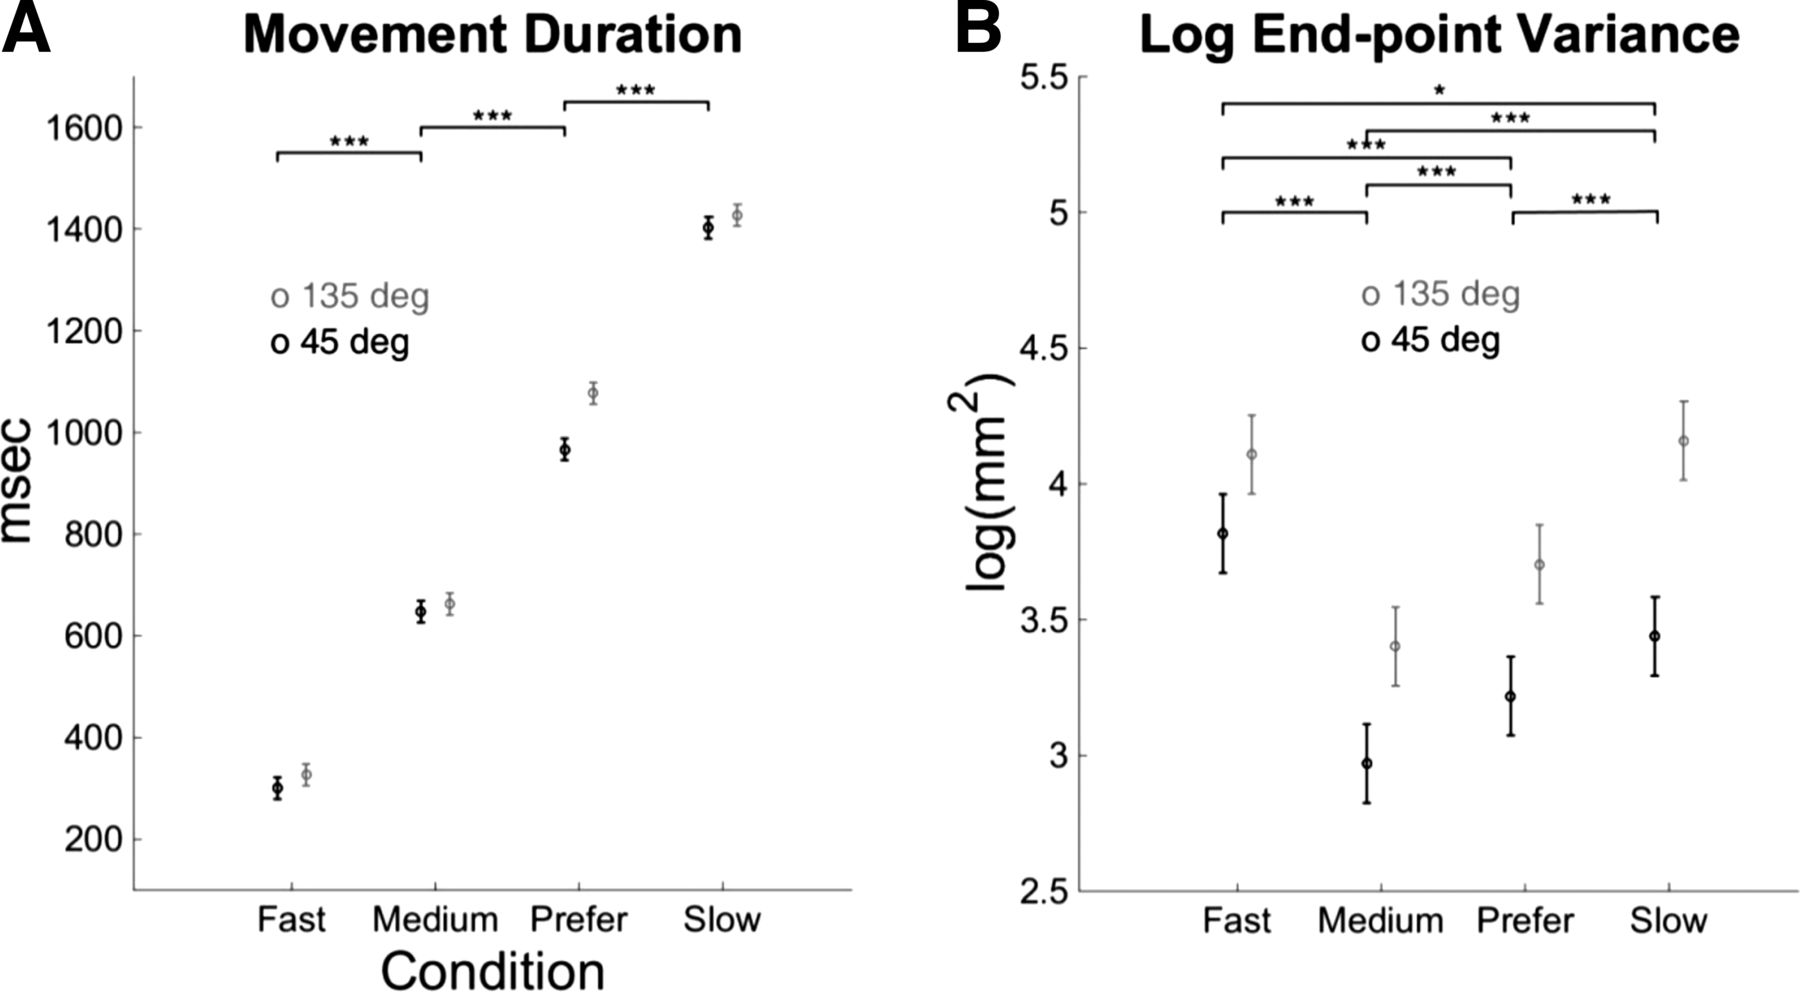
\includegraphics[width=0.8\linewidth]{figures/MT-data}
	\caption[Movement duration and endpoint movement variability]{Movement duration and endpoint movement variability in each condition for the \ang{45} and \ang{135} targets across subjects. A: movement duration in the 4 conditions for both targets. B: natural logarithm of endpoint variance in the 4 conditions for both targets. Both panels show estimated fixed effect coefficients with their confidence intervals in a model using mixed models with condition and target as main effects and target × condition interactions; see text for details. Asterisks show significance of difference between conditions for both targets (Bonferroni corrected): *P $<$ 0.05, ***P $<$ 0.0005; see text for additional comparison results.}
	\label{fig:mt-data}
\end{figure}


Mixed-model analysis shows significant fixed effects of condition and target on the (logarithm of) total endpoint variance (both with P $<$ 0.0001) as well as a significant condition $\times$ target interaction (P = 0.003). Endpoint variance was lowest for the medium duration (Figure \ref{fig:mt-data} B). Notably, for both targets, total endpoint variance in the medium movement duration condition was smaller than that in the preferred condition (P $<$ 0.0001). Total variance in the fast condition was greater than in the three other conditions (P$<$0.0001, P$<$ 0.0001, and P = 0.029 for medium, preferred and slow conditions, respectively). Variance in the slow condition was greater than variance in the preferred and medium conditions (P $<$ 0.0001 for both).

For all conditions, variance was greater for the \ang{135} target
than for the \ang{45} target (all P $<$ 0.0001). For the \ang{45} target, all differences between conditions were significant (P $<$ 0.0001), except for variance between fast and slow conditions, for which P = 1. For the \ang{135} target, all differences were significant at P $<$ 0.001, except for the differences between preferred and medium, which was significant at P = 0.015, and between preferred and slow, which was significant at P = 0.027.

\section{Discussion}

It has long been known that the duration of arm movements has an effect on endpoint variability \cite{Fitts1954, Woodworth1899}, but the relationship had not been systematically characterized. The present study provides two valuable additions to our understanding of movement planning.

First, our results show that, in arm reaching movement without visual feedback, an intermediate movement duration minimizes endpoint variability. Such minimum of endpoint variability was previously found in saccadic movements \cite{VanBeers2008} but, to our knowledge, not in arm reaching movements. Kinematic variability in human motion originates from a number of sources \cite{Faisal2008} (Faisal et al. 2008). In particular, the noise in individual motor neurons is well approximated by signal-dependent noise (see rationale in \cite{Harris1998}). However, noise in the final motor command departs from signal-dependent noise because this aggregate command combines the activities of many motor neurons distributed over multiple muscles. It is in particular possible that cocontraction yields a departure from signal-dependent noise. As a result, studies aimed at identifying the properties of noise in the motor commands of saccades \cite{VanBeers2007} and arm movements \cite{VanBeers2004} found that the noise is best characterized as a combination of signal-dependent noise and constant noise, with constant noise making a substantial contribution. With these two sources of noise, signal-dependent noise increases endpoint variability for short movement durations and constant noise increases variability for long movement durations by inducing a drift in final position.

The variability in task execution caused by the inherent noisiness of the neuromuscular system can be reduced by feedback mechanisms. In our experiment, movements were performed without vision, and thus only proprioceptive feedback was available to the subjects. 
The effect of proprioceptive feedback on movements appears small for movements at normal speed (see, e.g., Fig. 4 in \cite{Franklin2007}). However, for slower movements the effect of such feedback on endpoint error may become more important, especially with vision. Future work will be needed to compare variability with and without vision at different and self-chosen speed.

Second, our results show that the durations of reaching movements chosen by our subjects were longer than the durations minimizing endpoint variance. Thus, unlike what has been suggested for arm movements [Harris and Wolpert 1998, 2006], natural movements without vision at self-selected speed do not minimize variance. The longer preferred durations than the duration that minimizes variance may be due to effort minimization, which tends to lengthen movement duration. Our between-target results, as well as those from previous studies (e.g., Gordon et al. 1994; Park et al. 2016) showing that subjects slowed down for movements toward the \ang{135} target, which require greatest (estimated) effort because of greater inertia at the hand (see \cite{Schweighofer2015}), are consistent with this view.

We therefore propose that movement duration is determined by minimizing both variability and effort in the context of signal-dependent noise and constant noise in the motor command. In optimal control models of movements, the duration is determined to minimize antagonistic factors. In previous models, effort and signal-dependent noise were considered as factors to lengthen movement duration, and cost of time \cite{Hoff1994} and temporal discounting \cite{Haith2012, Rigoux2012, Shadmehr2010} were considered as a factor to shorten it. However, if we consider that constant noise is responsible for greater variability in slow movements, no additional factor is needed to shorten movement time. Instead, using a combination of signal-dependent noise and constant noise, simultaneous minimization of effort and endpoint variability provides a parsimonious mechanistic explanation for the overall pattern of errors across the fast, medium, preferred, and slow movement durations. In future work, estimating effort for different targets and speeds via quantification of metabolic costs (e.g., \cite{Huang2012}) will be necessary to determine whether the minimization of variability and effort is sufficient to determine movement time.



% Research Topic 2
\outline{1}{Movement Duration Minimizes Variability and Effort Concurrently}
\chapter{Movement Duration Minimizes Variability and Effort Concurrently: An Optimal Control Model}
\label{cha:optimalcontrol}

\outline{2}{Introduction}
\section{Introduction}
Our previous work (Chapter \ref{cha:movementtime}, published \cite{Wang2016}) demonstrated through experimental data that 
(1) in arm reaching movement without visual feedback, an intermediate movement duration minimizes endpoint variability; 
(2) the durations of reaching movements chosen by our subjects were longer than the durations minimizing endpoint variance. 
\cite{Wang2016} proposed that 
(1) two kinds of execution noise, Constant (CN) and Signal-Dependent Noise (SDN), lead to endpoint variability respectively at long and short movement durations, hence the joint effects of CN and SDN result in an intermediate movement duration that minimizes endpoint variability;
(2) effort is also minimized together with endpoint variability, which drives subjects to choose a duration that is longer that the duration minimizing endpoint variability.

Hypothesis (1) expands previous works on effects of execution noise in motor planning and control.
\cite{Harris1998, Harris2006} used SDN and minimum endpoint variance to account for reaching movement planning and kinematics. 
However, their model cannot distinguish minimizing endpoint variability due to SDN from minimizing effort, because formulation of effort often\footnote{For example, when effort is defined as the integral of squared torque or motor commands} leads to equivalent mathematical expressions as endpoint variance \cite{Wang2016, OSullivan2009}. 
Moreover, since minimizing variability due to SDN slows down movement, they failed to explain subjects, given a specific task, do not move slower than they do to achieve smaller endpoint variability.
Since movements with longer duration have larger endpoint variability with the presence of CN \cite{Todorov2005}, our hypotheses consider CN as another component of execution noise, such that minimizing variability would yield a compromise between SDN and CN, leading to a specific movement duration. 
The level of CN estimated in \cite{VanBeers2004} to account for endpoint distributions was comparable with the level of SDN, showing that CN as an execution noise cannot be ignored.

Optimal control theory assumes that movements can be understood as the solution of an optimization process.
The cost function of this optimization process is generally composed of two parts: one encodes the goal of the movement; the other penalizes some inherent feature of the movement \cite{Diedrichsen2010}. 
The first part can be formularized as the endpoint variance \cite{Harris1998}, or the endpoint error \cite{Todorov2005}; 
the second part can be based on the integrated jerk \cite{Flash1985}, integrated torque change \cite{Uno1989}, or integrated squared motor commands \cite{Todorov2002} (which was what we used in this work). 
To our knowledge, The relationship between movement duration and the two parts of the cost function has not been examined systematically and thoroughly.
Our hypothesis (2) provides insights on the distinct role of movement variability (first part of the cost function) and effort (second part of the cost function) for determining the duration of a movement.

We tested our hypotheses in computer simulations using stochastic open-loop optimal control \cite{Todorov2005} model with CN and SDN as execution noise.  
Although $\sigma_{\text{SDN}}$ and $\sigma_{\text{CN}}$ (see equation \ref{eqn:cnsdn} have previously been estimated \cite{VanBeers2004}, these estimates were based on inverse dynamics control of a simulated arm with a viscosity parameter that was estimated at rest from restoring forces to small perturbations \cite{Gomi1998}. 
However, the amount of viscosity during movements is presumably substantially smaller during movement than at rest \cite{Burdet2013}. 
In addition, we found in simulations (results not shown) that viscosity has a profound effect on the distribution of endpoints.  
We therefore re-estimated $\sigma_{\text{SDN}}$ and $\sigma_{\text{CN}}$ as well as a free viscosity parameter by fitting an optimal open-loop controller to endpoint reaching data in Chapter \ref{cha:movementtime}.

We then used these parameters to simulate reaching movements, and investigated endpoint variability and effort of movement with different durations.
%Our results reveal distinct roles of CN, SDN, and effort in planning movements.

\outline{2}{Methods}
\section{Methods}
To test our hypothesis, we built an open-loop stochastic optimal control model with both SDN and CN, estimated the levels of CN and SDN through the matching of the model with data in Chapter \ref{cha:movementtime}, and simulated endpoint distributions and effort of movement with different movement durations.

\subsection{Open-loop Stochastic Optimal Control Model}
The reaching movement is simulated with a planar arm with a shoulder and an elbow, whose joint angles are represented by $\bm{q} = (q_1, q_2)^T$, controlled by the open-loop stochastic optimal controller. 
The forward and inverse kinematics are formulated as in \cite{VanBeers2004}, and the dynamics equation is

\begin{equation} \label{maindynamics}
	\ddot{\bm{q}} = \bm{M}(\bm{q})^{-1} (\bm{\tau} - \bm{C}(\bm{q}, \dot{\bm{q}}) - \bm{B}\dot{\bm{q}})
\end{equation}

where $\bm{M}(\bm{q})$ is the inertia matrix, $\bm{C}(\bm{q}, \dot{\bm{q}})$ accounts for the centrifugal force and the Coriolis effect, and $\bm{B}$ is the viscosity matrix, which we assume to be a diagonal matrix with a single value $b$ on the diagonal. $b$ is a free parameter as discussed above. 
See Supplemental Material \ref{app:kindyn} for matrices definitions and parameter values.

We use a second-order linear filter as the muscle model (as in \cite{VanBeers2004}) which receives motor commands and gives torques over joints:

\begin{equation}
	\bm{u} = t_et_a\ddot{\bm{\tau}} + (t_e+t_a)\dot{\bm{\tau}} +\bm{\tau}
\end{equation}

where $\bm{u}$ is the motor command, $t_e = 30$ ms, $t_a = 40$ ms are time constants representing excitation and activation respectively \cite{VanderHelm2000}. 

The motor command $\bm{u}$ is corrupted with signal-dependent noise and constant noise:

\begin{equation}\label{eqn:cnsdn}
u_t \rightarrow (1 + \epsilon\sigma_{\text{SDN}}) u_t + \xi\sigma_{\text{CN}}
\end{equation}

where $\epsilon$ and $\xi$ are random variables from the normal Gaussian distribution.
$\sigma_{\text{CN}}$ and $\sigma_{\text{SDN}}$ represent the levels of noise.

To circumvent the difficulty of solving a nonlinear optimal control problem, we discretized and linearized the kinematics and dynamics equations with 10 ms time step interval around an approximated solution (as in \cite{Li2004}, details shown in Supplemental Material \ref{ocformulation}), giving rise to a linear-quadratic problem with the following cost to minimize:

\begin{equation}\label{eqn:cost}
V = \bm{s}_T^T\bm{Q}_T\bm{s}_T + \sum_{t=1}^T\bm{u}_t^T\bm{Ru}_t
\end{equation}

where $\bm{s_t}$ is the state vector. 
$\bm{Q}$ is arranged in such a way that the first term represents the square of endpoint error in hand space (Supplemental Material \ref{app:cost}). 
$\bm{R}$ is a diagonal matrix with a single value $w_r$ on the diagonal.
$w_r$ is a free parameter.
The second term, the integral of squared motor commands, is assumed to be the effort being considered in the process of determining movement duration. 

\subsection{Endpoint Distribution from Gaussian Execution Noise}

As shown in equation \ref{eqn:cnsdn}, the execution noise (CN and SDN) are assumed independent and Gaussian. 
The endpoint distribution due to execution noise is generally not Gaussian due to nonlinearity of the kinematics and dynamics. 
Through linearization of the system, we essentially used Gaussian as an approximation of the actual endpoint distribution. 
This approximation makes the algorithm much more efficient (thanks to the covariance propagation equation, see Supplemental Material \ref{app:covarProp}), than simulating large number of trials and calculating statistics over the endpoints (seen in \cite{VanBeers2004,Guigon2008}).
In order to make sure this approximation is appropriate, we compared the distribution from the linearized system to the original nonlinear system. As shown in figure \ref{fig:linearizeddistributionapprox}, the Gaussian distributions given by the linearized system (the blue 95\% confidence ellipse) are good approximations of the actual distributions of the original nonlinear system (the 2-dimension histogram, from 6000 simulated endpoints).

\begin{figure}
	\centering
	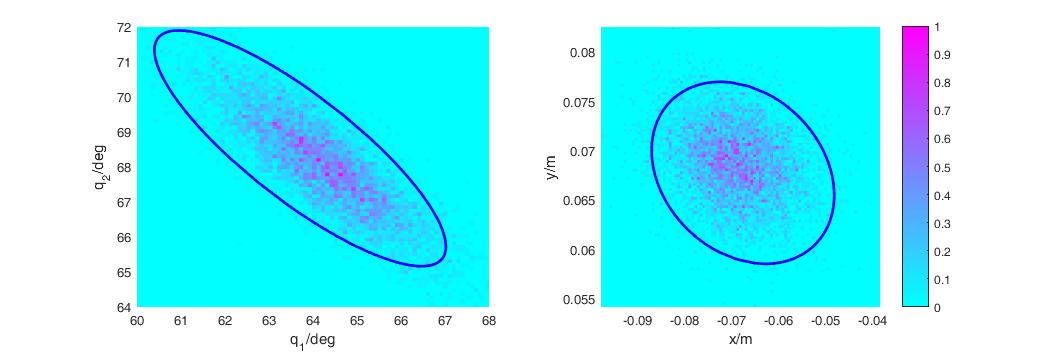
\includegraphics[width=\linewidth]{figures/linearizedDistributionApprox}
	\caption[Endpoint distributions of linearized system approximate the original]{Endpoint distributions of linearized system approximate the original. On the left is the distribution of joint angles at the endpoint position; on the right is the distribution of endpoints in task space. The blue 95\% confidence ellipses are distributions of linearized system; the 2-dimension histogram are distributions of the original system.}
	\label{fig:linearizeddistributionapprox}
\end{figure}

\subsection{Estimation of SDN and CN in Reaching Movements}
Although $\sigma_{\text{SDN}}$ and $\sigma_{\text{CN}}$ (see equation \ref{eqn:cnsdn}) have previously been estimated in \cite{VanBeers2004}, these estimates were based on inverse dynamics control of a simulated arm with a viscosity parameter that was estimated at rest from restoring forces to small perturbations \cite{Gomi1998}. 
However, the amount of viscosity during movements is presumably substantially smaller during movement than at rest \cite{Burdet2013}. 
In addition, we found in simulations (Supplemental Material \ref{app:oc}) that viscosity has a profound effect on the distribution of endpoints.  
We therefore re-estimated $\sigma_{\text{SDN}}$ and $\sigma_{\text{CN}}$ with viscosity as a free parameter by fitting an optimal open-loop controller to reaching data described in Chapter \ref{cha:movementtime}.

We picked the $\sigma_{\text{SDN}}$ and $\sigma_{\text{CN}}$ values that minimize the following fitting error function:

\begin{equation}
\label{eqn:fiterror}
\sum_{t}\sum_{c} (\text{TE}_{\text{data},t,c} - \text{TE}_{\text{sim},t,c})^2
\end{equation}

where $t$ and $c$ are indexes for target and condition, and TE stands for Total Error defined as 

\begin{equation}
\text{TE}_{\text{data}} = \frac1N\sum_n \left( (x - x^*)^2 + (y - y^*)^2 \right) 
\end{equation}

where $n$ is index for trials;

\begin{equation}
\text{TE}_{\text{sim}} = (\bar{x} - x^*)^2 + (\bar{y} - y^*)^2 + \text{tr}(\bm{P})
\end{equation}

where $(\bar{x},\bar{y})$ and $\bm{P}$ are the first (mean) and second (covariance matrix) central moment of the simulated endpoint distribution. 
The expressions of TE for data and simulation are different because $\text{TE}_{\text{data}}$ is calculated from actual endpoint data, whereas $\text{TE}_{\text{sim}}$ is calculated from the first and second moment of endpoint distribution.
We used \textsf{patternsearch} in Matlab to determine $\sigma_{\text{CN}}$ and $\sigma_{\text{SDN}}$ as well as viscosity parameter $ b $ that minimize the fitting error function \ref{eqn:fiterror}. 
In addition, we systematically varied $ w_r $ from $ 10^{-7} $ to 〖$ 10^{-5} $, but found that it had very little effect on both endpoint distributions and estimation of other three free parameters (at most 5\%). We therefore set $ w_r $ = $ 2\times 10^{-6} $ because larger values lead to inability of reaching to the target and smaller values decrease effect of effort minimization in movement generation. 
		
We found that for simulated movement that is longer than 1 second, the endpoint variability is very sensitive to CN.
We therefore assume $\sigma_{\text{CN}}$ depends on movement durations, but $\sigma_{\text{SDN}}$ is constant. [need rational and citation] 

With the estimated  $\sigma_{\text{CN}}$ and $\sigma_{\text{SDN}}$ as well as viscosity parameter $ b $, we simulated reaching movements to both targets with different movement duration.

\outline{2}{Results}
\section{Results}

\subsection{Estimation of SDN and CN in Reaching Movements}

The minimization of the fitting error function yielded the following noise and viscosity parameters: $\sigma_{\text{SDN}} = 0.298$ (unit-less), $\sigma_{\text{CN}}$(fast, medium, preferred, slow) = (0.010, 0.037, 0.035, 0.031)(\si{N.m}), and $b=0.110$ (\si{kg.m^2/s}). 
Note that our estimation of viscosity is significantly lower than \cite{VanBeers2004}. 

We interpolate $\sigma_{\text{CN}}$ as a function of movement duration using piecewise cubic Hermite interpolation \cite{Fritsch1980}, shown in figure \ref{fig:interpcn}.

\begin{figure}
	\centering
	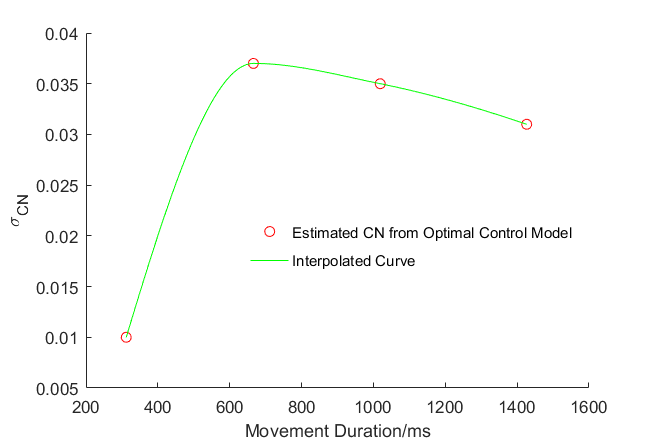
\includegraphics[width=0.75\linewidth]{figures/interpCN}
	\caption[Interpolation of $\sigma_{\text{CN}}$]{The Interpolation of $\sigma_{\text{CN}}$ against movement duration using piecewise cubic Hermite interpolation. The constant noise level is low at fast movement, and increases with movement duration, until it reaches a plateau.}
	\label{fig:interpcn}
\end{figure}

The model with estimated noise and viscosity parameters produces a Movement Duration - Total Error relationship that is very close to the data, shown in figure \ref{fig:total-error}.

\begin{figure}
	\centering
	\includegraphics[width=\linewidth]{"figures/total error"}
	\caption[Model with estimated parameters reproduces U curve relationship between Movement Duration and Total Error]{Model with estimated parameters reproduces U curve relationship between Movement Duration and Total Error. The model has 6 free parameters: four $\sigma_{\text{CN}}$ values for four movement durations,  $\sigma_{\text{SDN}}$, viscosity $ b $.}
	\label{fig:total-error}
\end{figure}



\subsection{Simulation of Cost vs. Movement Duration}

For both the \ang{45} and the \ang{135} targets, the stochastic optimal control model with parameters estimated above produced a U-shape relationship between total error and movement duration (Figure \ref{fig:variability---cost---minimum-shift}). 
The total error reached a minimum at an intermediate movement duration (approximately 600 ms for both targets), and increased either for faster or slower movements. 

The total cost (equation \ref{eqn:cost}) also exhibited a U-shape characteristic. 
For the left target, the total cost curve reached the minimum at about 1000 ms, very close to the average movement duration (1053 ms) that the subjects chose at the preferred condition. 
However, for the right target, the total cost curve reached the minimum at a movement duration only a little longer than the movement duration that minimizes the total error, not enough to the average movement duration (about 1000 ms) that the subjects chose at the preferred condition.
The difference stems from the larger effort required for a movement to the target at \ang{135} (which involves both shoulder and elbow rotation) than the target at \ang{45} (which involves roughly to an elbow rotation), as shown by the yellow curve in figure \ref{fig:variability---cost---minimum-shift}. 


\begin{figure}
	\centering
	\includegraphics[width=\linewidth]{"figures/variability - cost - minimum shift"}
	\caption[Simulation of Cost vs. Movement Duration Curve]{Simulation of Cost vs. Movement Duration Curve. The minimum of cost curve is at longer movement duration than the minimum of error curve, for both left and right target. The minimm of cost curve for the left target is at the "preferred" movement duration that the subjects choose in preferred condition (see Chapter \ref{cha:movementtime}); However, for the right target, the minimum of cost curve is not at the "preferred" movement duration.}
	\label{fig:variability---cost---minimum-shift}
\end{figure}

\outline{2}{Discussion}
\section{Discussion}
%If a task does not specifically (explicitely) have a varibility limit, then minimizing endpoint variance with SDN or minimizing effort inevitably leads to infinitely long movement duration. Therefore, additional mechanism is needed to reduce the movement duration. [Shadmehr 2010, 2016] proposes that the movement duration pose a discount of reward of the goal, which is called the "Cost of Time". Although Although this hypothesis has its base on physiological studies (Johnson  Bickel, 2002), but the discounting time constant is in the range of days or months. Whether discounting works within seconds remains to be confirmed. Another mechanism to reduce movement duration is to consider Constant Noise (CN). In Van Beers work, it has been shown that the effect of CN is not negligible ... and [authors] shows that CN in optimal control model, leads to larger variability at longer duration. Thus minimizing endpoint variability due to both signal-dependent and constant noise would yield a minimum that could determine movement duration. Correspondingly, our first hypothesis is that the CNS chooses intermediate reaching movement durations to minimize endpoint variability in the face of signal-dependent and constant noise.

It has long been known that the duration of arm movements has an effect on endpoint variability  \cite{Woodworth1899, Fitts1954}, but the relationship had not been systematically characterized. 
Our modeling results showed that, in coherence with data \ref{cha:movementtime}, an intermediate movement duration minimizes total endpoint error. 
Such intermediate movement duration was predicted by the presence of SDN and CN in the motor command and was previously found in saccadic movements \cite{VanBeers2008}, but had not been observed in reaching movements. 
In addition, the model showed that the minimization of endpoint variability and effort yields longer movement duration than minimizing only endpoint variability.
This behavior of the model, for a subset of movement direction (the \ang{135} target), is coherent with data in Chapter \ref{cha:movementtime}; however, the movement duration to the \ang{45} target was not well accounted for by the model. The effort required for the \ang{45} target, compared to the \ang{135} target, is very small, because the movement involves mostly only the elbow joint rotation. 
What's more, the use of squared motor command makes the effort decreases cubically with movement duration \cite{Shadmehr2016}, rendering the effect of effort very small to have an impact on the cost curve \ref{fig:variability---cost---minimum-shift}. 
We plan to use an optimal control model with an effort term in the cost function defined as the integral of absolute value of motor commands (which decreases linearly with movement duration).
It is reasonable to expect the effect of effort not so small at longer movement with a L1 norm effort term.
Nevertheless, our model supports the notion that effort is a determinant of movement planning in the context of SDN and CN on the motor command. 
Future work should aim at validating our estimate of effort e.g. via quantification of metabolic costs, e.g. \cite{Huang2012}.

Although minimum motor variability and minimum effort models appear conceptually different, \cite{OSullivan2009} pointed out that they are tightly related when only SDN is included: endpoint variance, which increases with SDN, corresponds to the effort deployed during the movement \cite{OSullivan2009}. 
Therefore, when considering either of these two factors, an additional term has to be considered in the cost minimized by the CNS to prevent selection of the slowest possible movements. 
It has for instance been proposed that subjects select such as the longest movement duration for which the hand is expected to land in the target with high probability \cite{Hoff1994,Harris1998,Harris2006}, or use temporal discounting of reward \cite{Shadmehr2010, Rigoux2012, Haith2012}. Our model does not require such additional factor to explain our data.
Instead, using a combination of SDN and CN, with the standard deviations of these two noise sources directly identified from reaching data in the first experiment, the model provides a parsimonious mechanistic explanation for the overall pattern of errors across the fast, medium, and slow movement durations.  
Future work will be needed to dissociate the effects of constant noise and discounting, in both movements with and without vision.

A further contribution of our study is the re-estimation of the contributions of $\sigma_{\text{SDN}}$ and $\sigma_{\text{CN}}$ in reaching movements. 
$\sigma_{\text{SDN}}$ has been estimated according to the force produced during isometric muscle contraction \cite{Jones2002, Slifkin1999} in saccadic movements, and in pointing movements without visual feedback \cite{VanBeers2004}. $\sigma_{\text{CN}}$ has been estimated in saccadic movements \cite{VanBeers2008} and pointing movements without visual feedback using a feedforward control model \cite{VanBeers2004}. 
Here, re-estimation of the noise parameter in arm reaching movements by setting viscosity as a free parameter yielded greater $\sigma_{\text{SDN}}$ compared to $\sigma_{\text{N}}$ than previously thought. We found $\sigma_{\text{SDN}}$ = 0.298 (unit-less) and $\sigma_{\text{CN}}$ $\sim$ 0.01-0.04 (N m), compared to $\sigma_{\text{SDN}}$ = 0.103 and $\sigma_{\text{CN}}$= 0.185 (N m) in \cite{VanBeers2004}. 

Van Beers et al. added to CN and SDN a third noise source called “temporal noise”, which was not needed in our model to account for the data. 
Note, however, that proprioceptive feedback was not taken into account both in van Beers’s and in our model, notably because the effect of such feedback on movements seem small for movements at normal speed (see e.g. Figure 4 in \cite{Franklin2007}). 
However, for slower movements the effect of such feedback on endpoint error may become more important – thus, the effect of such feedback would be to decrease the slope of the rightward portion of the U curves in simulations of Figure \ref{fig:variability---cost---minimum-shift}. 
As a result, the preferred movement times and the movement times that minimize variance in the model would be longer and, therefore, more in line with those of the experimental results. 
However, this would not modify the result that, in the context of SDN and CN, effort determines movement duration.


\section{Supplemental Material on Stochastic Control Modeling}
\label{app:oc}

\subsection{Kinematics and Dynamics}
\label{app:kindyn}
The forward kinematics, inverse kinematics and dynamics of this two-link arm model are widely used in the literature (e.g \cite{VanBeers2004}):

\begin{equation}
\bm{r} =\left(\begin{matrix} x\\y \end{matrix}\right) % = \text{FK}(\bm{q}) 
= \left[ \begin{matrix}  l_1\cos{q_1} + l_2\cos{(q_1+q_2)} \\ l_1\sin{q_1} + l_2\sin{(q_1+q_2)}  \end{matrix} \right]
\end{equation}
\begin{equation}
\begin{split}
& q_2 = \arccos{\left(\frac{r^2-l_1^2-l_2^2}{2l_1l_2}\right)} \\
& q_1 = \arctan{\left( \frac{y}{x} \right)} - \arctan{\left(\frac{l_2\sin{q_2}}{l_1+l_2\cos q_2 }\right)}
\end{split}
\end{equation}
\begin{equation} \label{dynamics}
\ddot{\bm{q}} = \bm{M}(\bm{q})^{-1} (\bm{\tau} - \bm{C}(\bm{q}, \dot{\bm{q}}) - \bm{B}\dot{\bm{q}})
\end{equation}

where $\bm{M}(\bm{q})$ is the inertia matrix, $\bm{C}(\bm{q}, \dot{\bm{q}})$ accounts for the centrifugal force and the Coriolis effect, and $\bm{B}$ is the viscosity matrix:

\begin{equation}
\bm{M} = \left( \begin{matrix} a_1 + 2a_2\cos\theta_2  &  a_3 + a_2 \cos\theta_2 \\
a_3 + a_2 \cos\theta_2   &  a_3
\end{matrix}\right)
\end{equation}
\begin{equation}
\bm{C} = \left( \begin{matrix} -\dot{\theta_2}(2\dot{\theta_1}+\dot{\theta_2}) \\
\dot{\theta_1}^2	\end{matrix} \right)
a_2\sin{\theta_2}
\end{equation}
\begin{equation}
\bm{B} = \left( \begin{matrix} b_1  & 0 \\ 0 & b_2 \end{matrix} \right)
\end{equation}
\begin{equation}
a_1 = I_1 + I_2 + m_2 l_1^2
\end{equation}
\begin{equation}
a_2 = m_2 l_1 s_2
\end{equation}
\begin{equation}
a_3 = I_2
\end{equation}

Arm length $\bm{l} = (l_1, l_2)^T$ = (30cm, 33cm), arm mass $m_i =$ (1.4kg, 1kg), $s_i=$ (11cm, 16cm) is the distance from the joint center to the center of the mass for link i , and $I_i$ = ($0.025\text{kgm}^2, 0.045\text{kgm}^2$) is the moment of inertia.

We use a second-order linear filter as the muscle model (as in Van Beers) which receives motor commands and gives torques over joints:

\begin{equation}
\bm{u} = t_et_a\ddot{\bm{\tau}} + (t_e+t_a)\dot{\bm{\tau}} +\bm{\tau}
\end{equation}

where $\bm{u}$ is the motor command, $t_e$, $t_a$ are time constants for excitation and activation respectively. 
The second order filter can be divided into two first order filter, respectively corresponding to excitation and activation:

\begin{equation}
\begin{split}
& \bm{u} = t_e \dot{\bm{e}} + \bm{e} \\
& \bm{e} = t_a \dot{\bm{\tau}} + \bm{\tau}
\end{split}
\end{equation}

All variables in \textbf{bold} letters (such as $\bm{e}$) have two components corresponding to shoulder and elbow.

The motor command $\bm{u}$ is corrupted with signal-dependent noise and constant noise:

\begin{equation}
u_t \rightarrow (1 + \epsilon\sigma_{\text{SDN}}) u_t + \xi\sigma_{\text{CN}}
\end{equation}

where $\epsilon$ and $\xi$ are random variables from the normal Gaussian distribution.
$\sigma_{\text{CN}}$ and $\sigma_{\text{SDN}}$ represent the levels of the noise.

\subsection{Optimal Control Formulation}
\label{ocformulation}

We choose Linear Quadratic Regulator (LQR) \cite{Li2004} to formulate the optimal control problem. Since the plant is nonlinear, a generalized LQR called iterative LQR (iLQR) is adopted here.

\paragraph{LQR with signal dependent noise.}
Standard LQR deals with independent Gaussian noise. To generalize to signal dependent noise (SDN) is quite straightforward. I conclude the result here.

Given the dynamics (linear) and cost function (sum of cost rate, quadratic), the problem is to get motor command $\bm{u}_t$ such that the cost function is minimized.
\begin{equation}\label{optimprob}
\begin{split}
\text{dynamics:~~} & \bm{x}_{t+1} = \bm{Ax}_t + \bm{Bu}_t + \bm{\xi}_t + \epsilon_t\bm{Cu}_t \\
\text{cost rate:~~} & \bm{x}_t^T\bm{Q}_t\bm{x}_t + \bm{u}_t^T\bm{Ru}_t
\end{split}
\end{equation}
$\bm{\xi}$ is the constant noise, $\epsilon\bm{Cu}$ is the signal dependent noise; $\bm{\xi}$ and $\epsilon$ are random variables. Specifically, $\epsilon$ is set to have unit standard deviation. Here I include only one source of SDN. To add more, simply add similar terms in the solution.

The solution is given by the following control policy:
\begin{equation}
\bm{u} = -(\bm{R}+(\bm{B+C})^T\bm{V}_{t+1}(\bm{B+C}) )^{-1} \bm{B}^T\bm{V}_{t+1}\bm{Ax}
\end{equation}
where $\bm{V}_t$ is the cost-to-go matrix 
\begin{equation}
\bm{V}_t = \bm{Q}_t + \bm{A}^T\bm{V}_{t+1}\bm{A} - \bm{A}^T\bm{V}_{t+1}\bm{B}(\bm{R} + (\bm{B+C})^T\bm{V}_{t+1}(\bm{B+C}))^{-1}\bm{B}^T\bm{V}_{t+1}\bm{A}
\end{equation}

\paragraph{Linearization}
To formulate the model in the form of LQR, a linearization is required. First is to discretize all time-dependent variables :
\begin{equation}
\begin{split}
\bm{q}_{t+1} &= \bm{q}_{t} + \dot{\bm{q}_{t}} \Delta t \\
\dot{\bm{q}}_{t+1} &= \dot{\bm{q}}_{t} + \ddot{\bm{q}}_{t} \Delta t \\
\bm{\tau}_{t+1} &= \bm{\tau}_{t} + \dot{\bm{\tau}_{t}} \Delta t \\
\bm{e}_{t+1} &= \bm{e}_{t} + \dot{\bm{e}_{t}} \Delta t \\
\end{split}
\end{equation}
The only nonlinear part is $\ddot{\bm{q}}_t$, in another word, $\dot{\bm{q}}_{t+1}$ is a nonlinear function of $\bm{q}_t$, $\dot{\bm{q}}_t$, ${\bm{\tau}}_t$, ${\bm{e}}_t$. Define the state vector 
\begin{equation}
\bm{x}_t=\left[ \begin{matrix}\bm{q}_t \\ \dot{\bm{q}}_t \\ \bm{\tau}_t \\ \bm{e}_t \end{matrix} \right]
\end{equation}
The linearized dynamics appears to be
\begin{equation}
\bm{x}_{t+1} - \tilde{\bm{x}}_{t+1} = \bm{A}_t (\bm{x}_t - \tilde{\bm{x}}_{t}) + \bm{B}(\bm{u}_t - \tilde{\bm{u}}_t)
\end{equation}
where $\tilde{\bm{x}}_t$ and $\tilde{\bm{u}}_t$ is any pair set of state and command, and matrix $\bm{A}_t$, as following, is evaluated at $\tilde{\bm{x}}_t$:
\begin{equation}
\bm{A}_t = \left[\begin{matrix}
1 & 0 & \Delta t & 0  & 0 & 0 & 0 & 0 \\
0 & 1 & 0 &\Delta t   & 0 & 0 & 0 & 0 \\
0 & \frac{\partial{\dot{q}_1^{t+1}}}{\partial{q_2^t}} & \frac{\partial{\dot{q}_1^{t+1}}}{\partial{\dot{q_1}^t}} & \frac{\partial{\dot{q}_1^{t+1}}}{\partial{\dot{q_2}^t}} & \frac{\partial{\dot{q}_1^{t+1}}}{\partial{\tau_1^t}} & \frac{\partial{\dot{q}_1^{t+1}}}{\partial{\tau_2^t}}& 0& 0 \\
0 & \frac{\partial{\dot{q}_2^{t+1}}}{\partial{q_2^t}} & \frac{\partial{\dot{q}_2^{t+1}}}{\partial{\dot{q_1}^t}} & \frac{\partial{\dot{q}_2^{t+1}}}{\partial{\dot{q_2}^t}} & \frac{\partial{\dot{q}_2^{t+1}}}{\partial{\tau_1^t}} & \frac{\partial{\dot{q}_2^{t+1}}}{\partial{\tau_2^t}}& 0& 0 \\
0 & 0 & 0 & 0   &   1-\frac{\Delta t}{t_a} & 0 & \frac{\Delta t}{t_a} & 0 \\
0 & 0 & 0 & 0   &   0 & 1-\frac{\Delta t}{t_a} & 0 & \frac{\Delta t}{t_a} \\
0 & 0 & 0 & 0   &   0 & 0 & 1-\frac{\Delta t}{t_e} & 0 \\
0 & 0 & 0 & 0   &   0 & 0 & 0 & 1-\frac{\Delta t}{t_e} \\
\end{matrix}\right]
\end{equation}
\begin{equation}
\bm{B} = \left[\begin{matrix}
0 & 0 \\
0 & 0 \\
0 & 0 \\
0 & 0 \\
0 & 0 \\
0 & 0 \\
\frac{\Delta t}{t_e} & 0 \\
0 & \frac{\Delta t}{t_e} 
\end{matrix}\right]
\end{equation}
Now the dynamics equation can be written as
\begin{equation}\label{dynam}
\begin{split}
\bm{x}_{t+1} &= \bm{A}_t \bm{x}_t + \bm{B}\bm{u}_t + \bm{c}_t \\
\bm{c}_t &= \tilde{\bm{x}}_{t+1} - \bm{A}_t\tilde{\bm{x}}_{t} - \bm{B}\tilde{\bm{u}}_t
\end{split}
\end{equation}

\paragraph{Cost Function}
\label{app:cost}
Usually there are two terms in the cost function; one is the cost for motor command $\bm{u}$, the other is for endpoint error $\bm{x} - \bm{x}^*$. To make both of them representable in quadratic form, $\bm{x}^*$ has to be imbedded into the state vector, so the new state vector is now defined as
\begin{equation}
\bm{x}_t=\left[ \begin{matrix}\bm{q}_t \\ \dot{\bm{q}}_t \\ \bm{\tau}_t \\ \bm{e}_t \\
\bm{q}^* \\ \dot{\bm{q}}^*
\end{matrix} \right]
\end{equation}
To make a quadratic cost function, the matrix $\bm{Q}$ must take the following form:
\begin{equation}
\bm{Q} = 
\left( \begin{matrix}
\bm{I}_{4\times4} \\
\bm{0}_{4\times4} \\
\bm{-I}_{4\times4} 
\end{matrix} \right)
\bm{J}^T
\left( \begin{matrix}
w_p &&&\\
&w_p&& \\
&&w_v&\\
&&&w_v 
\end{matrix} \right)
\bm{J}
\left( \begin{matrix}
\bm{I}_{4\times4} &
\bm{0}_{4\times4} &
\bm{-I}_{4\times4} 
\end{matrix} \right)
\end{equation}
where $w_p$ and $w_v$ are weights for position error and velocity error respectively, and $\bm{J}$ is the Jacobian matrix. The matrices $\bm{A}$ and $\bm{B}$ in dynamics equation also change:
\begin{equation}
\begin{split}
\bm{A} & \leftarrow \left( \begin{matrix}
\bm{A} \\
&\bm{I}_{4\times4} \\
\end{matrix} \right) \\
\bm{B} & \leftarrow \left( \begin{matrix}
\bm{B} \\
\bm{0}_{4\times2} \\
\end{matrix} \right)
\end{split}
\end{equation}
In conclusion, the result of linearization is the following LQR problem:
\begin{equation}\label{linlqr}
\begin{split}
\text{dynamics:~~}\bm{x}_{t+1} =& \bm{A}_t \bm{x}_t + \bm{B}\bm{u}_t + \bm{c}_t \\
(\text{where~~~}\bm{c}_t = & \tilde{\bm{x}}_{t+1} - \bm{A}_t\tilde{\bm{x}}_{t} - \bm{B}\tilde{\bm{u}}_t) \\
\text{cost:~~~~~~~~~~~} & \bm{x}_T^T\bm{Q}_T\bm{x}_T + \sum_{t=1}^T\bm{u}_t^T\bm{Ru}_t \\
\end{split}
\end{equation}

\paragraph{Iterative LQR}
The solution to equation \ref{linlqr} is not the solution to the original nonlinear problem, since it is just a linear approximation around $\tilde{\bm{x}}_t$ and $\tilde{\bm{u}}_t$. However, the solution can be taken as a new start point, and so on. When the iteration converges, the solution to equation \ref{linlqr} is $\tilde{\bm{u}}_t$ itself.

\paragraph{Covariance Matrix Propagation}\label{app:covarProp}
Once we get the optimal solution $\tilde{\bm{u}}$ from iterative LQR, we can plug it back into equation \ref{linlqr} (the same as the dynamics equation \ref{dynam}) to get the optimal trajectory. We can also turn on SDN in a form that is consistent with equation \ref{optimprob}, and/ or any form of constant noise, to simulate arm movement with motor/ state noise. The statistics of multiple simulations then can be compared with experiment data.

Many works look at the characters of endpoint distributions of arm reaching movement \cite{VanBeers2004, Guigon2008}. Instead of running repetitively the simulations, there is another way to get the endpoint distribution, namely to calculate the covariance matrix of the state vector after each time step. Let us consider equation \ref{dynam} with motor command $\bm{u}_t$ corrupted with constant noise (CN) and signal dependent noise (SDN). That is,
\begin{equation}
u_t \rightarrow (1 + \epsilon\sigma_{\text{SDN}}) u_t + \xi\sigma_{\text{CN}}
\end{equation}
where $\epsilon$ and $\xi$ are random variables with normal distribution, $\sigma$ represents the standard deviation of the motor noise. We also assume that the noise of different components of $\bm{u}$ are independent from each other, though they share the standard deviation. We have,
\begin{equation}
E[\bm{u}_t\bm{u}_t^T] = 
\left(\begin{matrix}
\sigma_{\text{CN}}^2 + 		\sigma_{\text{SDN}}^2 u_{1t}^2   &  0 \\
0  &   \sigma_{\text{CN}}^2 + 		\sigma_{\text{SDN}}^2 u_{2t}^2   \\
\end{matrix}\right)  \equiv \bm{Q}_t
\end{equation}
I omit the mean of the variables for simplicity. Apply to the dynamics equation \ref{dynam}, Let $\bm{P}_t = E[\bm{x}_{t}\bm{x}_{t}^T]$ we have
\begin{equation}
\bm{P}_{t+1} = \bm{A}_t \bm{P}_t\bm{A}_t^T + \bm{B}\bm{Q}_t\bm{B}^T
\end{equation}

\subsection{Results}\label{results}
\paragraph{Effects of Viscosity}
In \cite{VanBeers2004}, The viscosity matrix $\bm{B}$ in equation \ref{dynamics} is set to be diagonal with a value of 0.8 Nms/rad:
\begin{equation}
\bm{B} = 
\left(\begin{matrix}
0.8 & 0 \\
0 & 0.8 \\
\end{matrix}\right)
\end{equation}
Here I compare simulation results with \cite{VanBeers2004} value and a value of zero.

For a movement to a 90 degree target, simulation with high viscosity value gives S-shaped trajectory and asymmetric velocity profile  (figure \ref{fig:0.8}), whereas simulation with zero viscosity gives bell shaped velocity profile (figure \ref{fig 0.0}).
\begin{figure}[h]
	\centering
	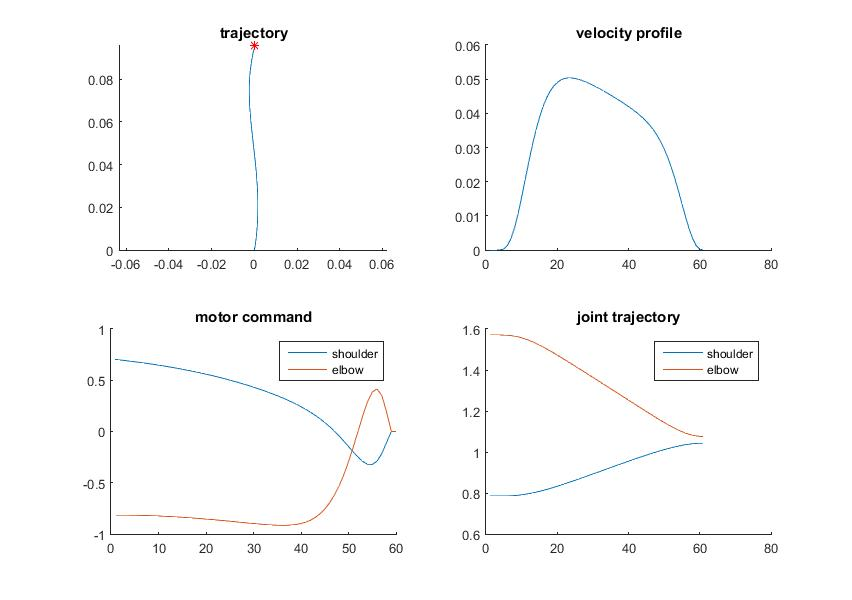
\includegraphics[width=\textwidth]{up8} 
	\caption{simulation result with high viscosity value}
	\label{fig:0.8}
\end{figure}
\begin{figure}[h]
	\centering
	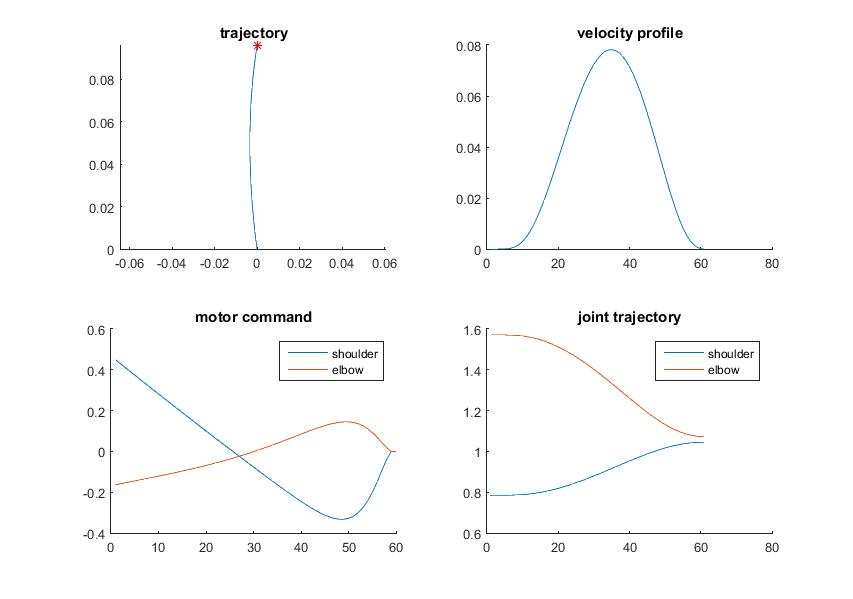
\includegraphics[width=\textwidth]{up0}
	\caption{simulation result with zero viscosity value}
	\label{fig 0.0}
\end{figure}





% Research Topic 3
\outline{1}{Learning is Modulated by Joint Synergies, Whereas Recovery is Modulated by Redundancy Exploration in Robotic Training Post-Stroke}
\chapter{Learning is Modulated by Joint Synergies, Whereas Recovery is Modulated by Redundancy Exploration in Robotic Training Post-Stroke}
\label{cha:armeospring}



\outline{2}{Introduction}
\section{Introduction}
Stoke is one of the leading cause of death and disability globally today (Benjamin et al., 2017).
Movement impairment due to stroke affects quality of life of stroke survivors (cite).
Stroke survivors usually display atypical movement patterns, referred to as abnormal “synergies” (Brunnström, 1970). 
It is not clear how abnormal synergies interact with the recovery of function. 
On the one hand, abnormal joint coordination may serve as compensation mechanism for functional daily use (Levin, Kleim,  Wolf, 2009); 
on the other hand, it is not clear how this compensation mechanisms helps or hinders recovery. 
To improve rehabilitation effectiveness, a better understanding of how joint coordination patterns affect recovery of functional abilities is required.
 
The challenging of stroke rehabilitation also stems from a character of high variability in lesion, impairment, spontaneous recovery, and responsiveness to therapy (Cramer, 2008a, 2008b). 
It is therefore crucial to recognize individual differences and identify key factors that play important role for recovery.
 
Due to the redundant nature of upper extremity kinematics, healthy individuals exploit redundancy (Kutch  Valero-Cuevas, 2011) or control the task relevant part of the redundancy to achieve a certain task (Scholz  Schöner, 1999). 
(Singh, Jana, Ghosal,  Murthy, 2016) shows that redundancy in joint space is exploited by healthy individuals to facilitate learning. 
For individuals post-stroke however, it is unclear what roles redundancy might play in motor learning and recovery.
 
In this study, we investigate the effect of abnormal synergy patterns and redundancy exploitation on motor learning and recovery. 
We use Principal Component Analysis (PCA) to quantify joint synergies (van Kordelaar, van Wegen,  Kwakkel, 2012) and measure similarities between synergies with principle angles between subspaces (Björck  Golub, 1973). 
We adapt the method in (Singh et al., 2016) to estimate redundancy exploitation.
 

\outline{2}{Methods}
\section{Methods}

\subsection{Data Collection}

\textbf{Participants.} 
We recruited 11 young (age 23 $\pm$ 2) healthy subjects (7 males) as the control group.
We recruited 53 post-stroke individuals with gender and affected side balanced, shown in table \ref{tab:demog}. 
Participants receive conventional rehabilitation besides robot-aided rehabilitation.

\begin{table}[b]
	\begin{tabular}{c c c c c c c c}
		\hline
		Group & No. & Age & Affected Side & Gender & FM(0-66) & Post Stroke Days & No. of Tests\\
		\hline
		Stroke & 53 & 59$\pm$14 & 29L, 24R & 19F, 30M & 25$\pm$9 to 39$\pm$ 14 & 56$\pm$21 & 80 in 4 weeks \\ 
		Control & 11 & 23$\pm$2 & - & 4F, 7M & - & - & 20 in 1 weeks \\
		\hline
	\end{tabular}
	\caption{Participants information}
	\label{tab:demog}
\end{table}

\textbf{Device.}
Our robot-aided rehabilitation uses Armeo@Spring exoskeleton from Hocoma\footnote{https://www.hocoma.com/us/} for therapy training. 
Shown in figure \ref{fig:1setupschedule}, the exoskeleton has 6 degrees of freedom, summarized in table \ref{tab:devicedof} and Fig. \ref{fig:1setupschedule}B. 
It is attached to the arm by two or three velcro straps. 
The exoskeleton has two springs equipped, at the upper arm and the forearm respectively. 
The springs can be adjusted to compensate the gravity force of the arm. 
Lengths of the exoskeleton are also adjustable to adapt to user's arm length.
There are no motors at any joints; user has to move actively to control the exoskeleton. 
User's trunk is mildly constrained by the velcro strap at the upper arm.


\begin{table}
	\begin{tabular}{c c c c}
		\hline
		Joint No. & Joint Name & Anatomical Counterpart & Direction \\
		\hline
		1(a) & Inner Shoulder Angle & Shoulder Horizontal Ab-/Adduction & Left/Right \\
		1(b) & Outer Shoulder Angle & Shoulder Horizontal Ab-/Adduction & Left/Right \\
		2 & Upper Arm Angle & Shoulder Flex-/Extension & Up/Down \\
		3 & Elbow Angle & - & Left/Right \\
		4 & Forearm Angle & - & Up/Down \\
		5 & Pro-/Supination Angle & Pro-/Supination & - \\ 
		6 & Flex-/Extension Angle & Wrist Flex-/Extension & - \\
		\hline
	\end{tabular}
	\caption{Degrees of freedom of ArmeoSpring exoskeleton.}
	\label{tab:devicedof}
\end{table}

The device records all joint angles (that is, the joints of the exoskeleton), and calculates the end effector location through a forward kinematics model of the exoskeleton. 
The end effector location then is used to control a cursor on a screen, displayed vertically in front of the user. 
All joint angles and end effector locations are recorded.

\textbf{Training and Test.}
Participants in the control group receive two training sessions (morning and afternoon) for five consecutive days in a week.
Post-stroke participants receive the same amount of training per day every weekday for four consecutive weeks (Fig. \ref{fig:1setupschedule}C).

One training session consists of several games; each lasts at most 3 minutes (with the exception of the ladybug pointing test mentioned below).
One training session typically lasts about 20 minutes.

A ladybug-pointing test is scheduled at the beginning and the end of each training session. 
This test is two-dimensional; the movement along the dimension perpendicular to the screen is ignored. 
In this test, the user tries to catch ladybugs that appear one by one pseudo randomly on the screen. 
The sequence of locations that ladybugs appear is fixed, although within a test they seem random.
To catch the ladybug, the user moves the cursor to its location. 
The user has limited time to catch the ladybug.
After a ladybug is caught, or the time limit is reached, the ladybug disappears and the next ladybug appears somewhere else. 


\begin{figure}
	\centering
	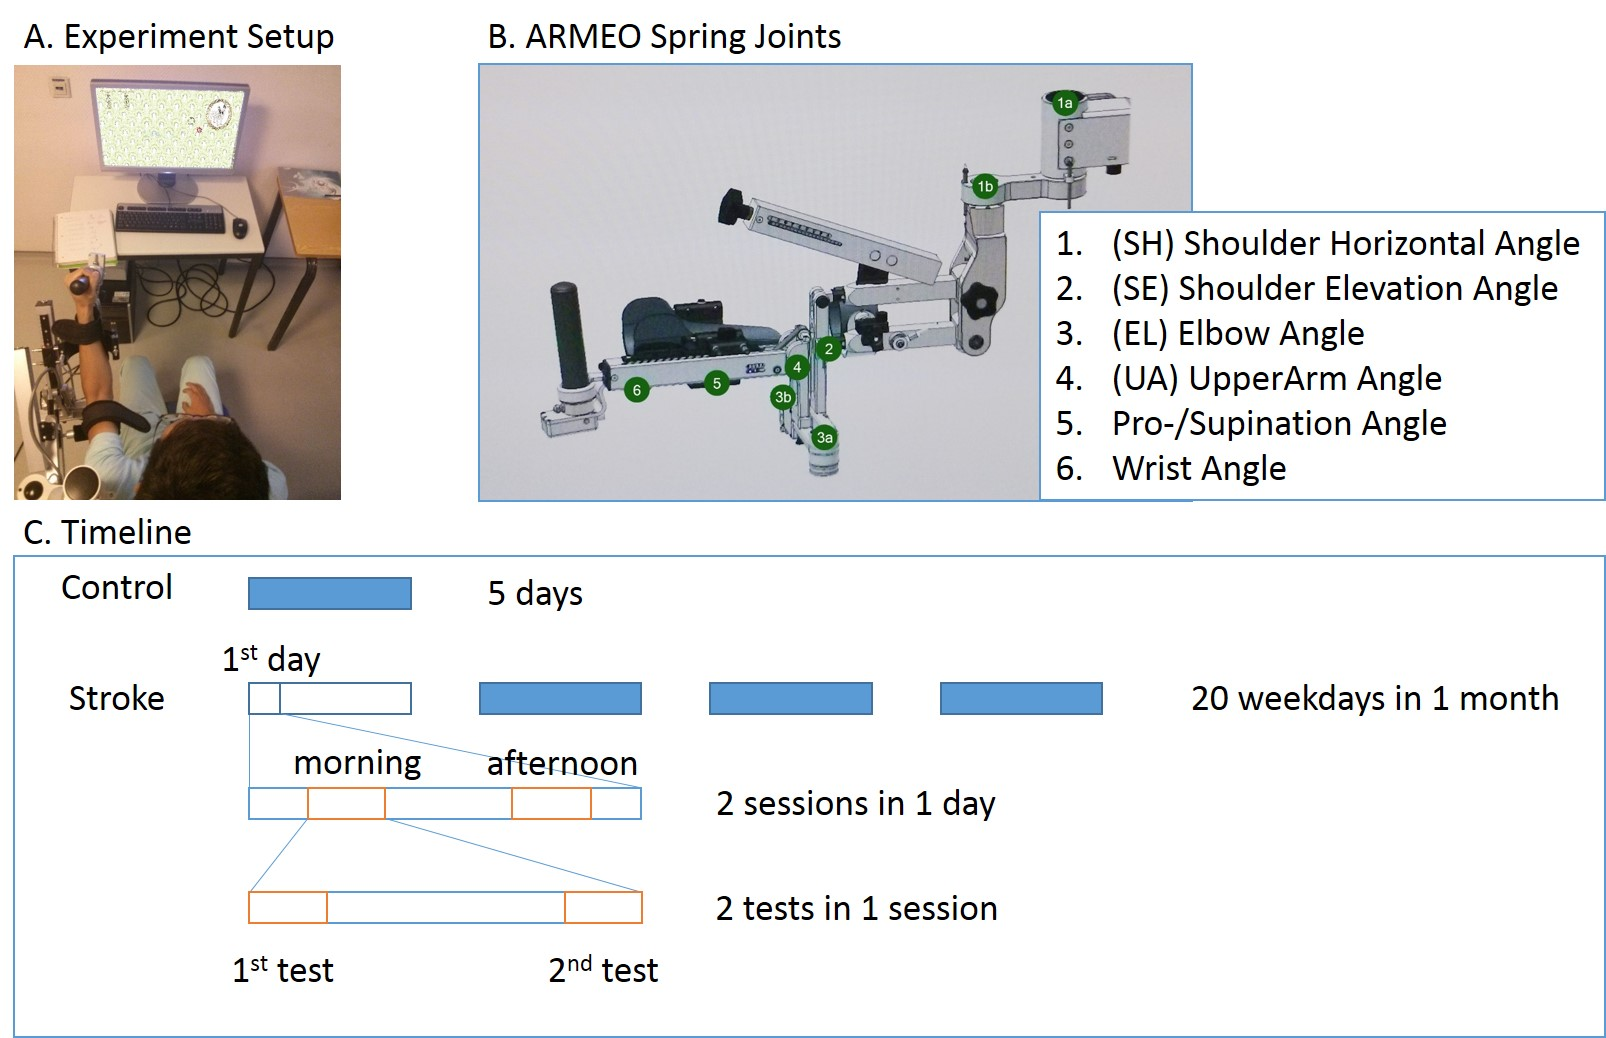
\includegraphics[width=1\linewidth]{figures/1setup&schedule}
	\caption[Experiment Setup and Schedule]
	{Experiment Setup, ARMEO Spring and Schedule. 
		A. Participants sit in front of a vertical screen on which the training games are displayed. In the ladybug test, the cursor responds to movements on a vertical plane. 
		B. Joints of ARMEO Spring. Summation of 1a and 1b is Shoulder Horizontal (SH) angle; 2 is Shoulder Elevation (SE) angle; 3a (only activated for right arm) and 3b (left arm) are elbow (EL) angles; 4 is ForeArm (FA) angle; 5 is pronation and supination angle; 6 is wrist angle.
		C. Two ladybug tests are administered at beginning and end of one session, two sessions are administered in morning and afternoon. Control group receives 5 days training, whereas stroke group receives 20 consecutive weekdays training.}
	\label{fig:1setupschedule}
\end{figure}

\subsection{Data Analysis}

\textbf{Preprocessing.}
We filter the data with a second order Butterworth filter with a cutoff frequency of 5 Hz.
We define a trial as the movement between two consecutive ladybugs.
A trial is considered successful if it starts from previously caught target and leads to the catching of next target. 
Only successful trials (control 99.8\%, stroke 78.2\%) are included in task space performance analysis.
We also exclude tests in which participants caught less than 25\% ladybugs (that is 0.7\% of all tests).

\textbf{Task Space Performance.}
We characterize task space performance of a ladybug test via the average number of peaks in the velocity profile \cite{}. 
To calculate the number of peaks in a velocity profile of a trial, we take the derivative of velocity (tangential acceleration) and count the number of times it goes from positive to negative.
We then take the average of number of peaks ($ p $) of all successful trials in the test.

We model the dynamics of number of peaks $ p $ as exponential functions of time $ t $ represented by task number, with mixed effects.
For participants in the control group, we consider a single exponential formulation
\begin{equation}\label{eqn:singleexp}
p_{i,j} = A_i \exp(-B_i t_{j}) + 1 + \epsilon_{i,j}
\end{equation}
where $ t_{j} = j $ is the test number $ j $, 
$ A_i $ is the mixed-effect coefficient representing the amplitude of the exponential for participant $ i $,
$ B_i $ is the mixed-effect coefficient representing the learning rate,
and $ \epsilon_{i,j} $ is the residual. 
We choose an asymptote of 1 because it is the theoretical limit of number of peaks.

For participants in the stroke group, we consider two exponential components to formulate the number of peaks
\begin{equation}\label{eqn:doubleexp}
p_{i,j} = A^f_{i,j} \exp(-B^f_{i,j} t_j) + A^s_{i,j} \exp(-B^s_{i,j} t_j) + 1 + \epsilon_{i,j}
\end{equation}
where $ A^f, A^s, B^f $ and $ B^s $ are constraint to be positive, and $ B^f > B^s $, therefore the first term represents a fast component, the second a slow component.

Mixed effect model coefficients are estimated via Matlab 2016a function \textsf{nlmefit}.

\textbf{Conversion of Joint Angles}
The recordings from ARMEO Spring are joint angles of the exoskeleton, different from anatomical joint angles.
It is therefore important to infer anatomical joint angles from exoskeleton joint angles. 

\textbf{Joint Space Variability.}
Because the last two joints (pronation/supination and wrist angle) have relatively small variance (control 12.4\%, stroke 4.6\%), we ignore them during joint space variability analysis and synergy analysis.
To quantify joint space variability and its relevance to the task space, we use a nonlinear forward kinematics model of the exoskeleton (cite company \cite{})
	\begin{equation}\label{eqn:nonlinearForwardKinematics}
	\bm{r} = f(\bm{\theta})
	\end{equation}
where $ \bm{r} = (x,y)^T $ is the location of the end effector, $ \bm{\theta} $ is joint angles (see Table \ref{tab:devicedof} and Fig. \ref{fig:1setupschedule}B for details). 
The distribution of variability for each target(ladybug) is calculated from the last 10 tests at the moment of catching the ladybug. 

The mean joint configuration across the last 10 tests at one specific ladybug ($ b $) is denoted by $ \bar{\bm{\theta}}_b $.
We will omit index $ b $ for convenience.
The Jacobian matrix at configuration $ \bar{\bm{\theta}} $ is obtained through forward kinematics (Eqn. \ref{eqn:nonlinearForwardKinematics})
	\begin{equation}
	\bm{J}(\bar{\bm{\theta}}) = \frac{\partial f(\bm{\theta})}{\partial \bm{\theta}} \Big\rvert_{\bar{\bm{\theta}}}
	\end{equation}
which is a 2 by 4 matrix.
The null space of Jacobian $ \bm{J} $ can be represented by basis of the space $ \bm{\xi}_i $, $ i= 1,2 $ which satisfy
	\begin{equation}
	\bm{J}(\bar{\bm{\theta}}) \bm{\xi}_i = 0
	\end{equation}
This means that movements in the null space ($ \bm{\xi}_i $) have no effect on the location of end effector, hence is task irrelevant.
Therefore we also call the null space as the task-irrelevant space.
For a specific test ($ t $) , the deviation of joint angles from $ \bar{\bm{\theta}} $ is
	\begin{equation}
	\Delta\bm{\theta}_t = \bm{\theta}_t - \bar{\bm{\theta}}
	\end{equation}
We will omit index $ t $ as well.
The projection of $ \Delta\bm{\theta} $ to the task-irrelevant space is
	\begin{equation}
	\Delta\bm{\theta}_{\text{null}} = \sum_i^m \langle \Delta\bm{\theta}, \bm{\xi}_i \rangle \bm{\xi}_i, m=2
	\end{equation}
where $ \langle,\rangle $ represents inner product.
In the end, we quantify the task-irrelevant variability by calculating the mean of squared $ \Delta\bm{\theta}_{\text{null}} $
	\begin{equation}\label{eqn:nullvar}
	V_{\text{null}}(t,b) = \mathbb{E}_{t,b} (\Delta\bm{\theta}_{\text{null}}^T\Delta\bm{\theta}_{\text{null}})
	\end{equation}
where $ t,b $ index tests and targets (ladybugs). 
We then average $ V_{\text{null}}(t,b) $ across tests ($ t $) and targets ($ b $) as the measure of task-irrelevant variability of a participant. 
Because $ V_{\text{null}} $ is similar to the calculation of variance, it has unit of $ \text{deg}^2 $.
It is on average the summation of variance across all joints.

To obtain variability in the orthogonal (task-relevant) space, we simply replace $ \bm{\xi}_i $ with the basis of the orthogonal space, $ \bm{\psi}_i $, $ i= 1,2 $  :
	\begin{equation}
	\Delta\bm{\theta}_{\text{orth}} = \sum_i^m \langle \Delta\bm{\theta}, \bm{\psi}_i \rangle \bm{\psi}_i, m=2
	\end{equation}
and the task-relevant space variability is
	\begin{equation}\label{eqn:taskvar}
	V_{\text{orth}}(t,b) = \mathbb{E}_{t,b} (\Delta\bm{\theta}_{\text{orth}}^T\Delta\bm{\theta}_{\text{orth}})
	\end{equation}

\textbf{Synergy Extraction and Analysis.}
We use Principal Component Analysis (PCA) to extract joint synergies from each ladybug test.
PCA belongs to a family of Dimension Reduction methods.
Principal Components of joint angles, which captures most of the variance presented in the data, can be interpreted as joint synergies \cite{}.
In this study, we only look at the first two synergies which on average account for 83.9\% joint angle variance for control group, 83.1\% for stroke group.
Joint synergies of healthy participants are quite stable across individuals.
We calculate the averaged synergies shown in figure \ref{fig:6synergy}C.

To evaluate the synergy pattern of stroke participant, we use the principal angle \cite{} between subspaces that are spanned by synergies \cite{}.
Generally, the principal angle $ \phi $ between two subspaces is the minimum rotation angle required to rotate one subspace onto the other.
A principal angle of \ang{0} indicates the same synergy patterns, whereas \ang{90} indicates completely different ones.
Therefore we refer to this angle as synergy abnormality.
We use Matlab 2016a \textsf{subspace} \cite{} to calculate the principal angle. 

For each stroke participant, we investigate the synergy abnormality (principal angle) $ \phi $ between his synergies from every test and the average healthy synergies.
$ \phi(t) $ ($ t $ for test) reflects the abnormality of participant's joint synergy patterns throughout training. 
We fit a linear mixed effect model to $ \phi(t) $ with a fixed effect on the intercept $ \phi(0) $ and a random effect on both the intercept and slope (we do not include a fixed effect on the slope because it is not significant when included in the model).
%The intercept $ \phi(0) $ tells us how different this participant's synergy pattern is initially different from the control group.
%It is therefore a measure of joint coordination prior training.

To investigate how joint synergies affects task space learning, we correlate $ \phi(0) $ with task space (fast and slow) learning rate.

\textbf{Linear Regression}
In this study, when doing linear regression, we identify outliers through Cook's Distance (Cook, 1977).
Instead of removing them, we adopt robust regression method with the bisquare weight function (Hoaglin, Mosteller, 1983).

\outline{2}{Results}
\section{Results}

Stroke participants show significant changes after training in kinematics performance.
Fig. \ref{fig:2stroketrajexamp} shows representative trajectories in both task space and joint space. 
After training, the trajectories in task space are straighter, and the joint trajectories also seem smoother. 
%In this particular trial in Fig. \ref{fig:2stroketrajexamp}B, the movement time is also shorter.


\begin{figure}
	\centering
	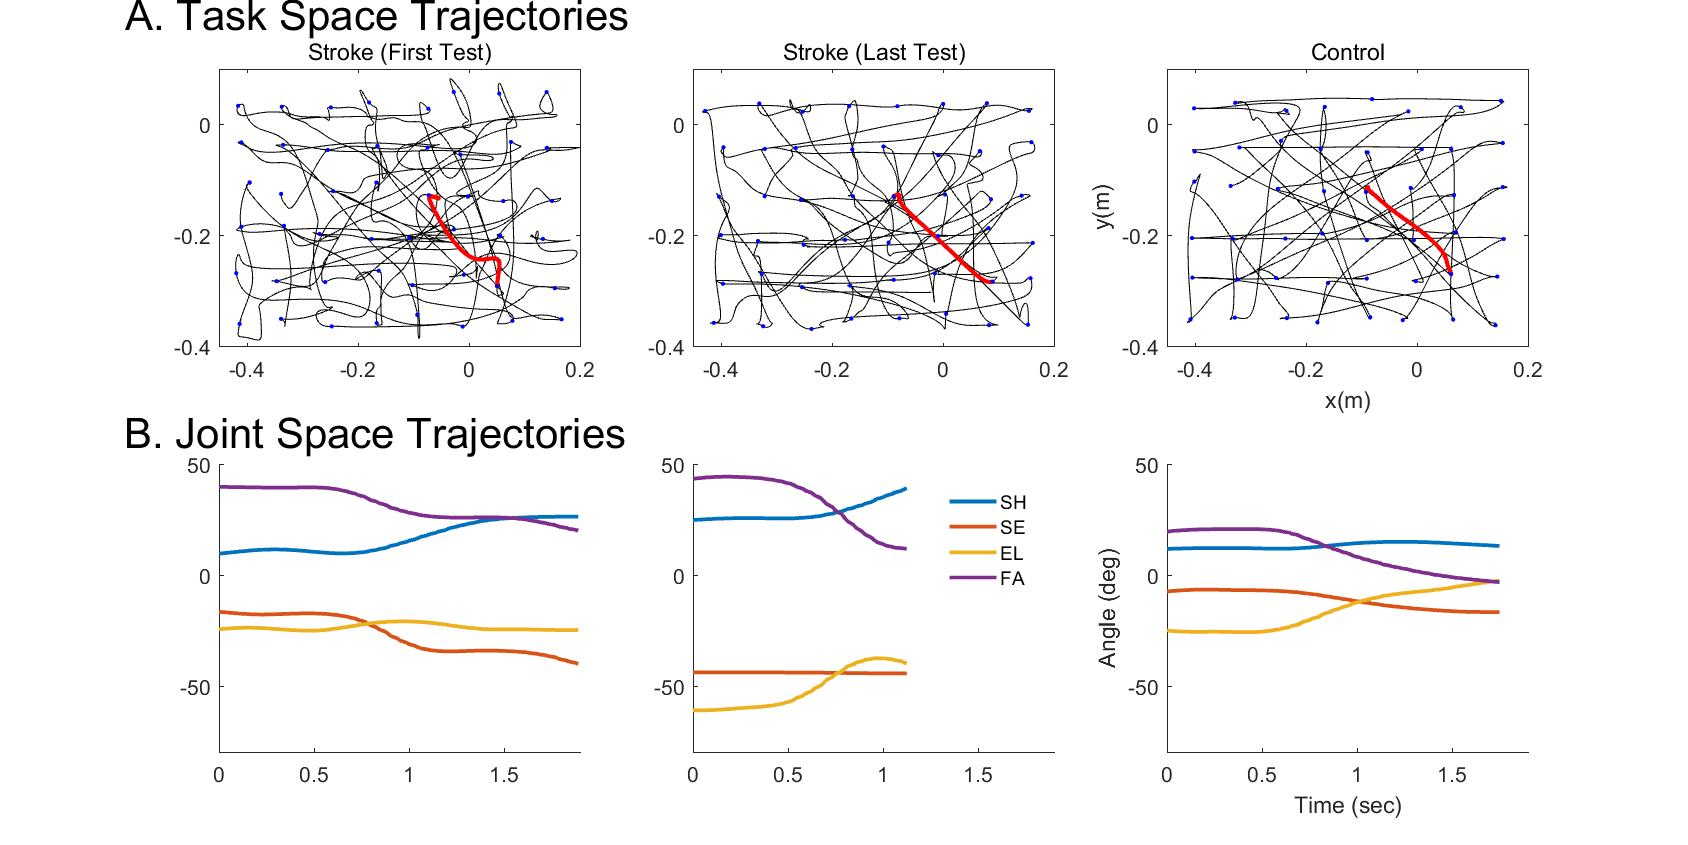
\includegraphics[width=1\linewidth]{figures/2strokeTrajExamp}
	\caption[Example trajectories]
	{Representative trajectories. 
		A. Representative task space trajectories. Trajectories after training are straighter.
		B. Representative joint space trajectories, correspond to the red part trajectories in panel A. Only the first four joints are shown.}
	\label{fig:2stroketrajexamp}
\end{figure}

\textbf{Task Space Performance.}
Fig. \ref{fig:3nopfixran} shows the number of peaks modeled by exponential functions.
Control subjects show much fewer number of peaks on average (Fig. \ref{fig:3nopfixran}A).
Stroke participants show significant improvement (Fig. \ref{fig:3nopfixran}B), although still more than control group at the end of training.


\begin{figure}
	\centering
	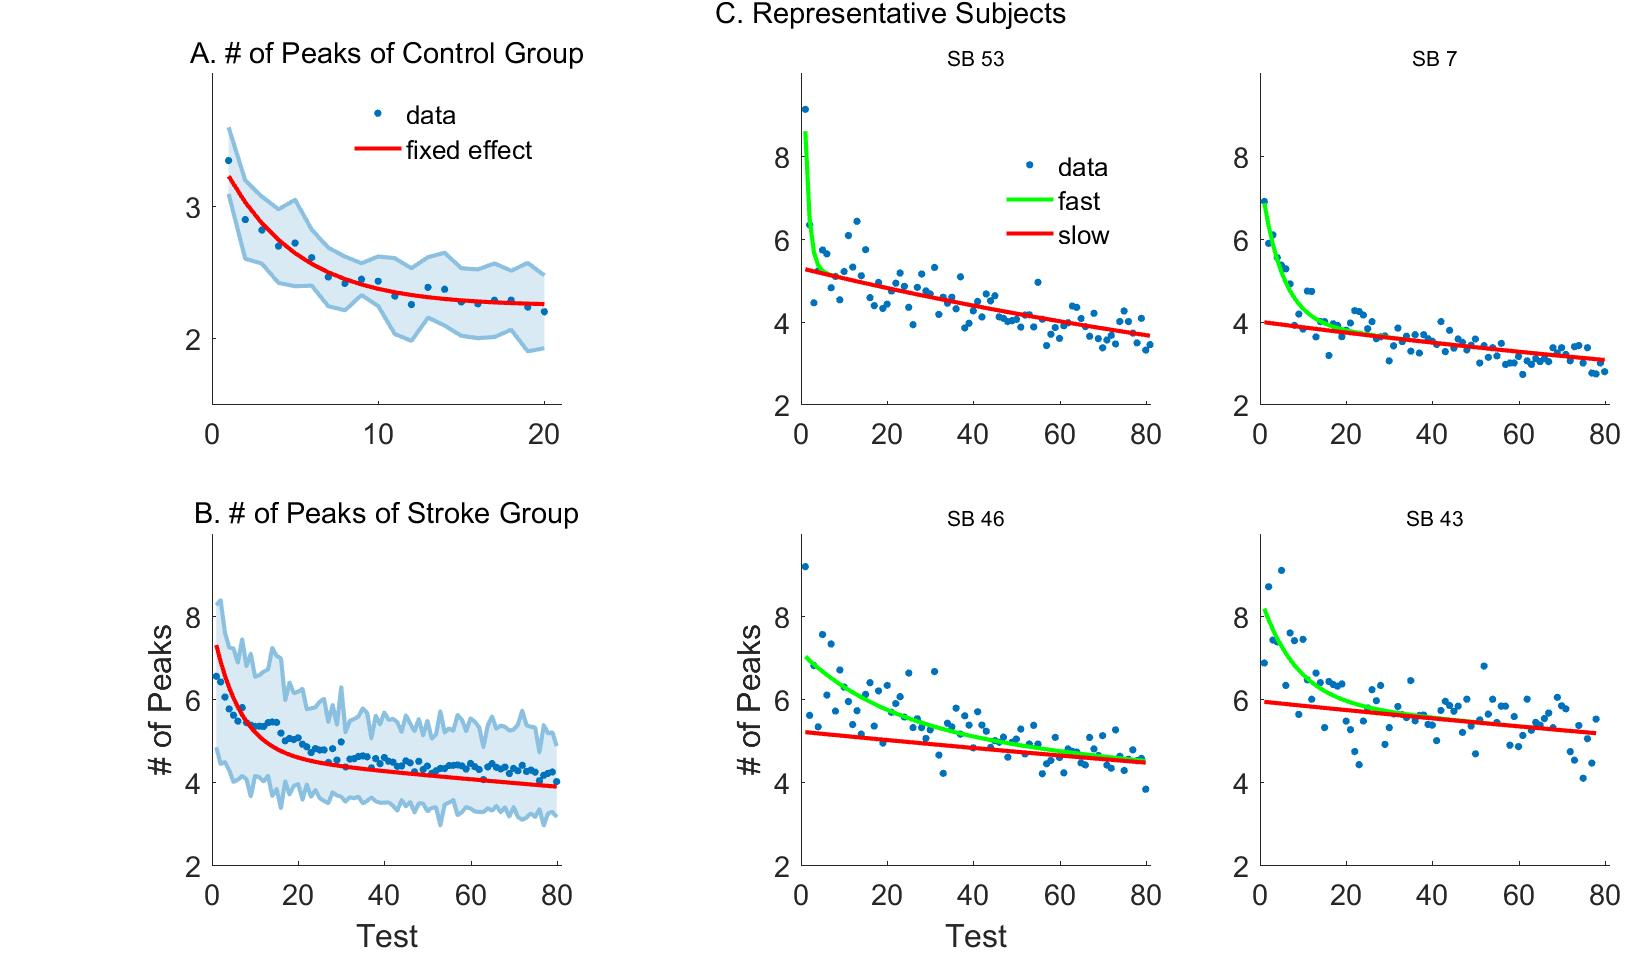
\includegraphics[width=1\linewidth]{figures/3nopFixRan}
	\caption[Double Exponential Model]
	{Double Exponential Model of Number of Peaks in Velocity Profile. 
		A,B: The fixed effect (group average) of the fitted exponential model of number of peaks. 
		Shaded area represents standard deviation;
		C: Representative participants.
		SB 53: fast learning rate and large task-irrelevant variability; 
		SB 46: slow learning rate and small task-irrelevant variability (see Fig. \ref{fig:5learnratevsnullvar} for task-irrelevant variability);
		SB 7: fast recovery rate and small initial synergy abnormality;
		SB 43: slow recovery rate and large initial synergy abnormality (see Fig. \ref{fig:6synergy} for initial synergy abnormality).
	}
	\label{fig:3nopfixran}
\end{figure}


The double exponential mixed effect model (Eqn. \ref{eqn:doubleexp}) gives two learning rates $ b_1 $ and $ b_2 $. 
We refer the smaller of the two, $ b_2 $ as the slow learning rate, the bigger, $ b_1 $ the fast learning rate.
Fig. \ref{fig:3nopfixran}C shows examples of individual fitting.
The slow component, due to small learning rate, is essentially linear; but the fast component usually goes to asymptote during the training.

To interpret these two fitted learning rates, we compare them with Fugul Meyer (FM) assessment score \cite{}.
The post training number of peaks and post training FM are significantly correlated ($ p = 0.0003 $, Fig. \ref{fig:4slowcomponentisrecovery}A).
This indicates that the number of peaks is a good measurement of abnormal synergy patterns.
In addition, the change of number of peaks before and after training due to the slow process (term $ a_2e^{-b_2t} $ in Eqn. \ref{eqn:doubleexp}), correlates significantly ($ p<0.0001 $) with the change of FM (Fig. \ref{fig:4slowcomponentisrecovery}B).
This further indicates that the slow learning process, rather than the fast one, reflects a recovery of synergy patterns.
We therefore refer to $ b_2 $ as the recovery rate, and $ b_1 $ as the learning rate.


\begin{figure}
	\centering
	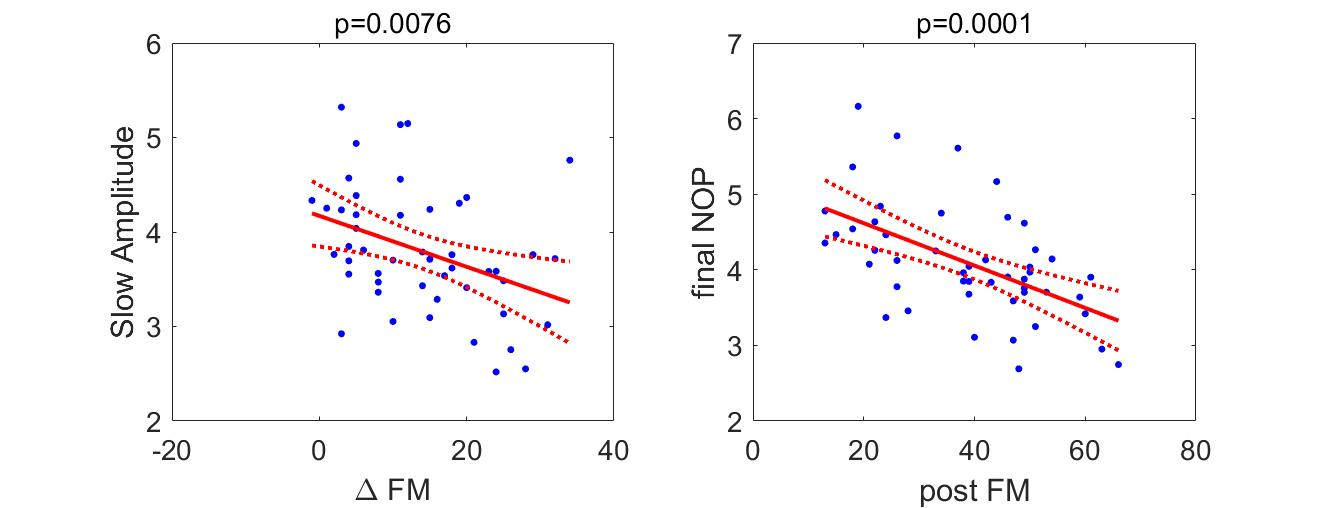
\includegraphics[width=1\linewidth]{figures/4slowComponentIsRecovery}
	\caption[Slow component corresponds to recovery as meaured by FM]
	{Slow component corresponds to recovery as measured by FM. 
		A: The number of peaks post training is correlated with FM post training;
		B: The change of number of peaks due to the slow process is correlated with the change of FM, prior and post training.
		The cyan regression line is normal least square regression; whereas the red regression line is robust regression with bisquare weight function. 
		Data points indicated by cyan crosses are outliers detected by Cook's distance.
	}
	\label{fig:4slowcomponentisrecovery}
\end{figure}

\textbf{Joint Space Variability.}
Both control group and stroke group display much larger task-irrelevant variability than task-relevant variability.
For example, for the control group, the task-irrelevant variability on average is $ \ang{18.3} \pm \ang{19.4} $ (measured by standard deviation, $ \sqrt{V_\text{null}} $); whereas the task-relevant variability ($ \sqrt{V_\text{orth}} $) on average is $ \ang{3.1} \pm \ang{2.9} $.

Task-irrelevant variability positively correlates with the learning rate $ b_1 $ (see Eqn. \ref{eqn:doubleexp}), as shown in Fig. \ref{fig:5learnratevsnullvar}.
Participants with small task-irrelevant variability learn slower (such as SB 46, see Fig. \ref{fig:3nopfixran}C: SB 46);
participants with large tasl-irrelevant variability learn faster (such as SB 46, see Fig. \ref{fig:3nopfixran}C: SB 53);


\begin{figure}
	\centering
	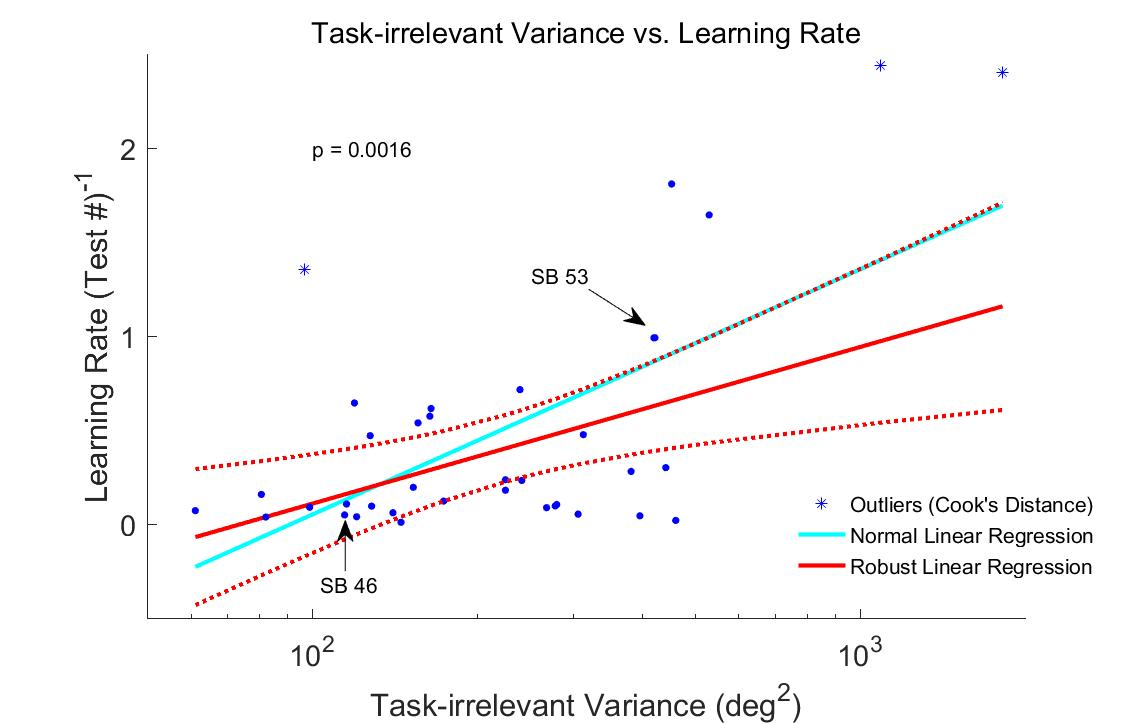
\includegraphics[width=1\linewidth]{figures/5learnRateVSnullVar}
	\caption[Exploration of Joint Redundancy facilitates learning]
	{Exploration of Joint Redundancy facilitates learning. 
		(The log of) null space variability is correlated with learning rate.
		SB 53 and 46 are representative participants, whose learning curves are shown in Fig.\ref{fig:3nopfixran}C.
		The cyan regression line is normal least square regression; whereas the red regression line is robust regression with bisquare weight function. 
		Data points indicated by cyan crosses are outliers detected by Cook's distance.}
	\label{fig:5learnratevsnullvar}
\end{figure}

\textbf{Synergy Analysis.}
We identify two synergies from control group, as shown in Fig. \ref{fig:6synergy}C.
The first synergy is composed of Shoulder Horizontal (SH) rotation and Elbow (EL) angle, and it is responsible for horizontal movements.
The second synergy is composed of Shoulder Elevation (SE) angle and Forearm (FA) angle, and it is responsible for vertical movements.

We are not able to identify stable synergies from stroke participants due to large differences across different participants.
They can share a similar structure as the control group (Fig. \ref{fig:6synergy}B), or have different structure (Fig. \ref{fig:6synergy}A).

The initial synergy abnormality correlates with the recovery rate $ b_2 $ (see Eqn. \ref{eqn:doubleexp}) as shown in Fig. \ref{fig:6synergy}D.
Participants with large abnormality recovers slower (such as SB 43, see Fig.\ref{fig:3nopfixran}C); while participants with small abnormality recovers faster (such as SB 7, see Fig.\ref{fig:3nopfixran}C).




\begin{figure}
	\centering
	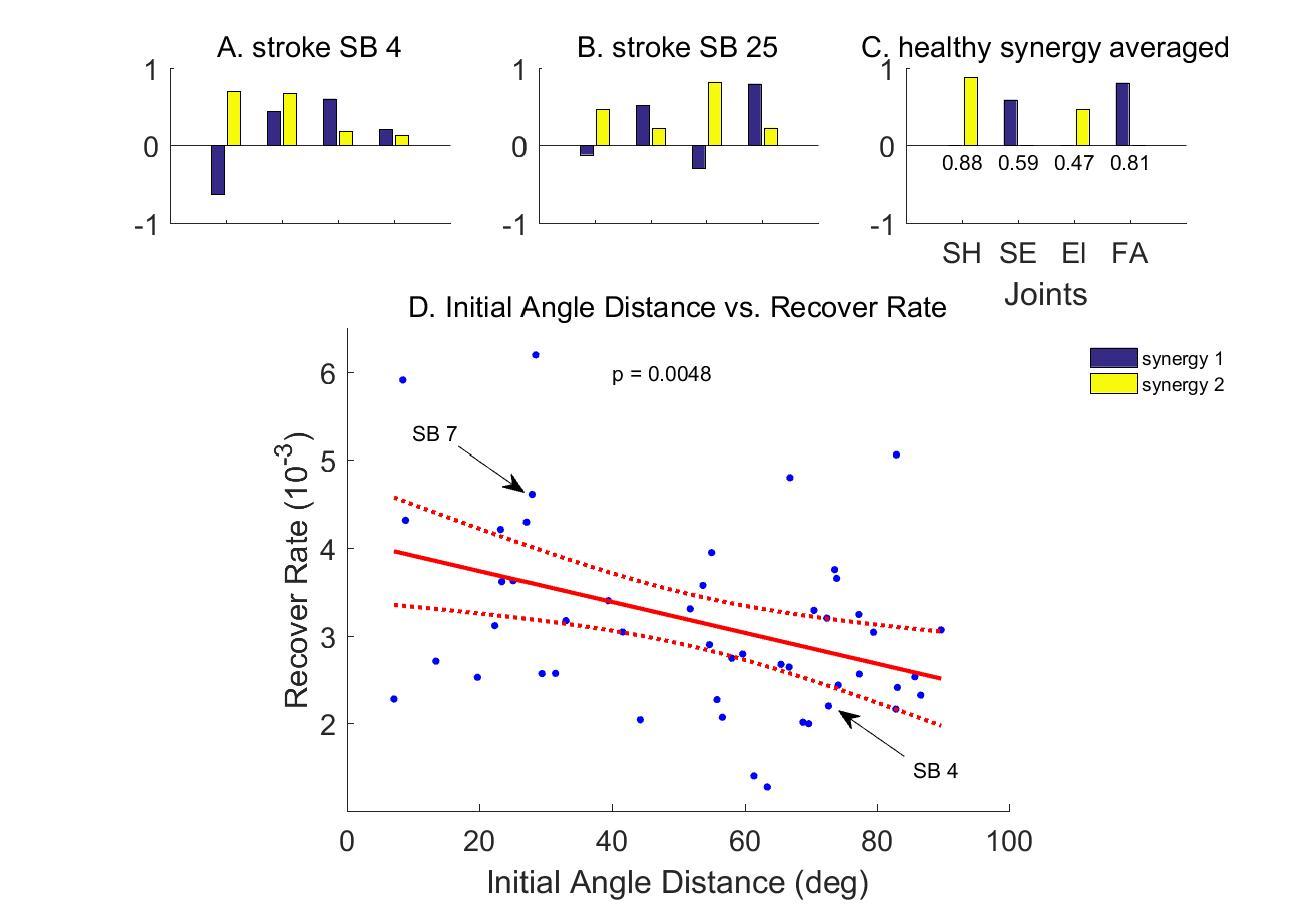
\includegraphics[width=1\linewidth]{figures/6synergy}
	\caption[Synergy Analysis]
	{Synergy Abnormality hinders recovery. 
		A-C. Radar plot of synergies. Dashed black line indicates zero. Blue and red lines are synergies.
		A. Representative participant with abnormal synergies;
		B. Representative participant with normal synergies. See Fig.\ref{fig:3nopfixran}C for their learning curves;
		C. Averaged synergies of participants in the control group;
		D. Synergy abnormality reduces recovery rate. SB 7 and 43 are representative participants, whose initial synergy patterns are shown in panel A and B, learning curves are shown in Fig.\ref{fig:3nopfixran}C.
		The cyan regression line is normal least square regression; whereas the red regression line is robust regression with bisquare weight function. 
		Data points indicated by cyan crosses are outliers detected by Cook's distance.}
	\label{fig:6synergy}
\end{figure}



\outline{2}{Discussion}
\section{Discussion}
We characterize kinematics performance with a double exponential model of number of peaks, and show evidence that the two components link to motor learning and recovery respectively. 
The mixed effect estimation of parameters allow us to obtain estimations of individual learning rates.

Task-irrelevant variability, or variance in the UnControlled Manifold (UCM), is a source of variability that doesn’t affect the execution of a task, which can be represented by variables. 
In the original study, (Scholz  Schöner, 1999) demonstrated that during a functional task, certain relevant variables are not controlled.
The redundancy of human arm kinematics dictates that there must be task-irrelevant variability (the variability that does not affect endpoint trajectories) in the joint space. 
We measure this task-irrelevant variability with adapted method from (Singh et al., 2016). 
Although this variability is task irrelevant, it is not unnecessary since it brings flexibility and allow versatile joint coordination for some specific task. 
However, how task-irrelevant variability affects learning (in healthy subjects) or recovery (in stroke survivors) is a question worth investigating. 
(Singh et al., 2016) suggested that this variability, as a form of redundancy exploitation, helps motor adaptation and learning. 
In our study, we found a correlation between task-irrelevant variability and learning rate of post-stroke individuals, suggesting that it also helps stroke individuals to learn a novel task.

Joint synergies are extracted through Principal Component Analysis (PCA). 
As a dimension reduction method, PCA provides components that explain the most variability in joint angle space. 
Along with other dimension reduction methods, PCA has been used to extract joint synergies (van Kordelaar et al., 2012). 
Similarities between synergies can be measured through the angle between two synergies in joint angle space, and similarities between groups of synergies can be measured through the angle between two subspaces (Bockemhl, 2010). 
We couldn’t verify the method used in (Bockemhl, 2010), instead we use numerical method in (Björck  Golub, 1973) to calculate angles between subspaces. 
A correlation between joint synergy abnormality and recovery rate may suggest that joint coordination patterns are important for functional recovery.



% Research Topic 4
\outline{1}{Diminishing Returns of Dose and Duration of Rehabilitation Post-Stroke as Revealed by Dynamic Mixed Effect Model}
\chapter{Diminishing Returns of Dose and Duration of Rehabilitation Post-Stroke as Revealed by Dynamic Mixed Effect Model}
\label{dosechapter}


\outline{2}{Introduction}
\section{Introduction}
In this chapter, I present my work on the data from the DOSE clinic trial.


\section{Method}
\subsection{DOSE Trial}
In this study, we analyzed the data from Dose Optimization for Stroke Evaluation (DOSE) clinical trial \cite{}. 
40 post-stroke individuals participated in this study. 
Fig.1 shows the timeline of the study: participants receive two baseline tests before three periods of therapy intervention, followed by 6 follow-up tests. 
Each period of therapy intervention lasts 1 week, right after a pre-training test and followed by a post-training test. 
There is one month between intervention periods and follow-up tests. 
The whole study lasts 37 weeks for each participant.
  
Participants were grouped randomly into four groups with different dosage of therapy training during the intervention period: zero, low, moderate, and high therapy dose, measured by the amount of time of treatment: 0, 5, 10, 20 hours per week.

In each test, participants received Wolf Motor Function Test (WMFT) and Bilateral Arm Reaching Test (BART), as well as an interview of Motor Activity Log (MAL). 
Concerning the BART and WMFT tests last as long as 2 hours, we include this testing effect into the hours of training, so that we have 22, 12, 7, 2 hours of training for the four groups.

\section{State Space Model to Nonlinear Mixed Effect Model}
In the field of motor perturbation adaptation, state space model is adopted to model learning behavior [cite]. 
In particular, the state of the system $ x_k $ at trial $ k $ follows 
\begin{equation}\label{ssm}
	x_{k+1} = Ax_k + Bu_k
\end{equation}
Where $ A $ represents retention, and often takes a value slightly smaller than 1; 
where as B, slightly bigger than 0, represents learning due to input $ u_k $ {often indicating the error in motor perturbation adaptation).
This formula can be written as a differential equation:
\begin{equation}
	\frac{\Delta x_k}{\Delta t} = \frac{x_{k+1}-x_k}{\Delta t} = \frac{(A-1)x_k}{\Delta t} + \frac{Bu_k}{\Delta t}
\end{equation}
Omit index $ k $ and let $ a = (A-1)/\Delta t $, $ b = B/\Delta t $ and $ \Delta t\rightarrow 0 $, we have
\begin{equation}\label{oode}
	\frac{dx(t)}{dt} = ax(t)+bu(t)
\end{equation}
The solution to this differential equation is in general
\begin{equation}\label{generalsolution}
	x = x_0e^{at} + b\int_0^t e^{a(t-\tau)}u(\tau)d\tau
\end{equation}
If $ a $ is small comparing to the time scale concerned (that is to say $ |at_{\text{max}}| \ll 1 $) and $ b $ is comparibly small to $ a $ (that is to say $ \text{lim}\frac{bu_\text{max}}{ax_\text{max}} \leqslant \text{const.} $), then the first order approximation to this solution is
\begin{equation}\label{specialsolution}
	x = x_0 + x_0at + b \int_0^t u(\tau)d\tau
\end{equation}
Let $ c=x_0 a $, the original differential equation \ref{oode} becomes
\begin{equation}
	\frac{dx(t)}{dt} = bu(t) + c
\end{equation}
To isolate the effect of training input $ u(t) $, we further assume that c can be ignored when $ u(t) \neq 0 $, i.e.
\begin{equation}\label{fode}
	\frac{dx(t)}{dt} = bu(t) + cv(t)
\end{equation}
where
\begin{equation}
v(t) = 
\begin{cases}
	1, & \text{if}\ u(t) = 0 \\
	0, & \text{otherwise}
\end{cases}
\end{equation}
Or, in logical notation, $ v(t) = \sim u(t) $. 
This assumption would be further justified later when we show $ bu(t) $ is much larger than $ c $.

Denote the solution to Eqn. \ref{fode} as nonlinear function $ x=f(x_0,b,c,t) $, we estimate the mixed effect model as
\begin{equation}\label{eqn:mixedeffect}
	x_i (t)=f(x_0i,b_i,c_i,t) + \epsilon_i (t)
\end{equation}
where $ x_0i $, $ b_i $, $ c_i $ are the mixed effect parameters which can vary from individual to individual (cite Bates).
$ \epsilon_i (t) $ is the residual. 
We choose different mixed effects on $ b_i $ and $ c_i $ to investigate different aspects of training mentioned above.

\textbf{Training Efficacy and Efficiency.}
To estimate the efficacy of training (the overall effect of training), we let $ u(t)=1 $ during the intervention periods as shown in Fig.2A. 
To estimate the efficiency of training (the effect of training per hour), we let $ u(t) $ to be the number of treatment hours corresponding to the group, as shown in Fig.2B. 
To investigate how training efficacy and efficiency depends on dosage of training, we use a linear formula for the mixed effects of $ b_i $ and $ c_i $:
\begin{eqnarray}
	b_i &=& \beta_1^b + \beta_2^b D_i + \delta_i^b   \\
	c_i &=& \beta_1^c + \beta_2^c D_i + \delta_i^c   \\
	x_{0i} &=& \beta_1^{x_0} + \beta_2^{x_0} F_i + \delta_i^{x_0}
\end{eqnarray}
where $ D_i $ is the dosage of training (number of hours per week) participant $ i $ received, 
$ F_i $ is the initial FM score of participant $ i $, 
$ \beta $ are fixed effects and $ \delta_i $ are random effects. 
Indexes on the shoulder indicates the parameter to which this fixed or random effect belongs.

In the case when we take the dosage of training as categorical variable, i.e. how efficacy and efficiency depends on the four groups, the formula becomes
\begin{equation}
	b_i = \beta_1^b + \beta_2^b D_{i2} + \beta_3^b D_{i3} + \beta_4^b D_{i4} + \delta_i^b
\end{equation}
Where $ D_{ij} $ is 1 when participant i belongs to group j, 0 otherwise. The formula for $ c_i $ is in the same structure.

\textbf{The Timing of Training}
To look at the effect of training at different period, we further assume $ b $ and $ c $ can take different values at different intervention periods. 
We applied this assumption in two ways: 1) A linear dependence of $ b $ (and $ c $) on training period $ k (k=1,2,3) $, namely
\begin{eqnarray}
	b(k) &=& b_0 + b_t (k-1) \\
	c(k) &=& c_0 + c_t (k-1)
\end{eqnarray}
So that we have two more parameters than Eqn. \ref{fode}. 

Due to insufficient data points (too few data points at each training period), we simplify the mixed effects of $ b(k) $ and $ c(k) $:
\begin{eqnarray}
	b_0 &=& \beta_1^b + \delta_i^b \\
	b_t &=& \beta_2^b
\end{eqnarray}
The formula for $ c_0 $ and $ c_t $ is in the same structure.

2) Independent values of $ b $ and $ c $ at different training period, namely
\begin{equation}
	b = b_k, c = c_k, k = 1,2,3
\end{equation}
So that we have four more parameters than Eqn. \ref{fode}. 

We use maximum likelihood to estimate parameters.


% Conclusion and ongoing work
\chapter{Conclusion and ongoing work}
\label{cha:conclusion}



\outline{1}{Reference List}
\begin{singlespace}
  % Bibliography
  \references{apalike}{references}
  \appendix
  % Appendices
%  \chapter{Supplimental Material on Stochastic Control Modeling}
\label{app:oc}

\section{Kinematics and Dynamics}
The forward kinematics, inverse kinematics and dynamics of this two-link arm model are widely used in the literature (e.g van Beers and ..):

\begin{equation}
	\bm{r} =\left(\begin{matrix} x\\y \end{matrix}\right) % = \text{FK}(\bm{q}) 
	= \left[ \begin{matrix}  l_1\cos{q_1} + l_2\cos{(q_1+q_2)} \\ l_1\sin{q_1} + l_2\sin{(q_1+q_2)}  \end{matrix} \right]
\end{equation}
\begin{equation}
	\begin{split}
	& q_2 = \arccos{\left(\frac{r^2-l_1^2-l_2^2}{2l_1l_2}\right)} \\
	& q_1 = \arctan{\left( \frac{x}{y} \right)} - \arctan{\left(\frac{l_2\sin{q_2}}{l_1+l_2\cos q_2 }\right)}
	\end{split}
\end{equation}
\begin{equation} \label{dynamics}
	\ddot{\bm{q}} = \bm{M}(\bm{q})^{-1} (\bm{\tau} - \bm{C}(\bm{q}, \dot{\bm{q}}) - \bm{B}\dot{\bm{q}})
\end{equation}

where $\bm{M}(\bm{q})$ is the inertia matrix, $\bm{C}(\bm{q}, \dot{\bm{q}})$ accounts for the centrifugal force and the Coriolis effect, and $\bm{B}$ is the viscosity matrix:

\begin{equation}
	\bm{M} = \left( \begin{matrix} a_1 + 2a_2\cos\theta_2  &  a_3 + a_2 \cos\theta_2 \\
										a_3 + a_2 \cos\theta_2   &  a_3
				\end{matrix}\right)
\end{equation}
\begin{equation}
	\bm{C} = \left( \begin{matrix} -\dot{\theta_2}(2\dot{\theta_1}+\dot{\theta_2}) \\
										\dot{\theta_1}^2	\end{matrix} \right)
				a_2\sin{\theta_2}
\end{equation}
\begin{equation}
	\bm{B} = \left( \begin{matrix} b_1  & 0 \\ 0 & b_2 \end{matrix} \right)
\end{equation}
\begin{equation}
a_1 = I_1 + I_2 + m_2 l_1^2
\end{equation}
\begin{equation}
a_2 = m_2 l_1 s_2
\end{equation}
\begin{equation}
a_3 = I_2
\end{equation}

Arm length $\bm{l} = (l_1, l_2)^T$ = (30cm, 33cm), arm mass $m_i =$ (1.4kg, 1kg), $s_i=$ (11cm, 16cm) is the distance from the joint center to the center of the mass for link i , and $I_i$ = ($0.025\text{kgm}^2, 0.045\text{kgm}^2$) is the moment of inertia.

We use a second-order linear filter as the muscle model (as in Van Beers) which receives motor commands and gives torques over joints:

\begin{equation}
	\bm{u} = t_et_a\ddot{\bm{\tau}} + (t_e+t_a)\dot{\bm{\tau}} +\bm{\tau}
\end{equation}

where $\bm{u}$ is the motor command, $t_e$, $t_a$ are time constants for excitation and activation respectively. 
The second order filter can be divided into two first order filter, respectively corresponding to excitation and activation:

\begin{equation}
	\begin{split}
	& \bm{u} = t_e \dot{\bm{e}} + \bm{e} \\
	& \bm{e} = t_a \dot{\bm{\tau}} + \bm{\tau}
	\end{split}
\end{equation}

All variables in \textbf{bold} letters (such as $\bm{e}$) have two components corresponding to shoulder and elbow.

The motor command $\bm{u}$ is corrupted with signal-dependent noise and constant noise:

\begin{equation}
u_t \rightarrow (1 + \epsilon\sigma_{\text{SDN}}) u_t + \xi\sigma_{\text{CN}}
\end{equation}

where $\epsilon$ and $\xi$ are random variables from the normal Gaussian distribution.
$\sigma_{\text{CN}}$ and $\sigma_{\text{SDN}}$ represent the levels of the noise.

\section{Optimal Control Formulation}\label{ocformulation}
We choose Linear Quadratic Regulator (LQR) \cite{todorov2006optimal} to formulate the optimal control problem. Since the plant is nonlinear, a generalized LQR called iterative LQR (iLQR) is adopted here.

\subsection{LQR with signal dependent noise}
Standard LQR deals with Gaussion noise that is independent. To generalize to signal dependent noise (SDN) is quite straight forward. I conclude the result here.

Given the dynamics (linear) and cost function (sum of cost rate, quadratic), the problem is to get motor command $\bm{u}_t$ such that the cost function is minimized.
\begin{equation}\label{optimprob}
	\begin{split}
	\text{dynamics:~~} & \bm{x}_{t+1} = \bm{Ax}_t + \bm{Bu}_t + \bm{\xi}_t + \epsilon_t\bm{Cu}_t \\
	\text{cost rate:~~} & \bm{x}_t^T\bm{Q}_t\bm{x}_t + \bm{u}_t^T\bm{Ru}_t
	\end{split}
\end{equation}
$\bm{\xi}$ is the constant noise, $\epsilon\bm{Cu}$ is the signal dependent noise; $\bm{\xi}$ and $\epsilon$ are random variables. Specifically, $\epsilon$ is set to have unit standard deviation. Here I include only one source of SDN. To add more, simply add similar terms in the solution.

The solution is given by the following control policy:
\begin{equation}
	\bm{u} = -(\bm{R}+(\bm{B+C})^T\bm{V}_{t+1}(\bm{B+C}) )^{-1} \bm{B}^T\bm{V}_{t+1}\bm{Ax}
\end{equation}
where $\bm{V}_t$ is the cost-to-go matrix 
\begin{equation}
	\bm{V}_t = \bm{Q}_t + \bm{A}^T\bm{V}_{t+1}\bm{A} - \bm{A}^T\bm{V}_{t+1}\bm{B}(\bm{R} + (\bm{B+C})^T\bm{V}_{t+1}(\bm{B+C}))^{-1}\bm{B}^T\bm{V}_{t+1}\bm{A}
\end{equation}

\subsection{Linearization}
To formulate the model in the form of LQR, a linearization is required. First is to discretize with Newton's method:
\begin{equation}
	\begin{split}
	\bm{q}_{t+1} &= \bm{q}_{t} + \dot{\bm{q}_{t}} \Delta t \\
	\dot{\bm{q}}_{t+1} &= \dot{\bm{q}}_{t} + \ddot{\bm{q}}_{t} \Delta t \\
	\bm{\tau}_{t+1} &= \bm{\tau}_{t} + \dot{\bm{\tau}_{t}} \Delta t \\
	\bm{e}_{t+1} &= \bm{e}_{t} + \dot{\bm{e}_{t}} \Delta t \\
	\end{split}
\end{equation}
The only nonlinear part is $\ddot{\bm{q}}_t$, in another word, $\dot{\bm{q}}_{t+1}$ is a nonlinear function of $\bm{q}_t$, $\dot{\bm{q}}_t$, ${\bm{\tau}}_t$, ${\bm{e}}_t$. Define the state vector 
\begin{equation}
	\bm{x}_t=\left[ \begin{matrix}\bm{q}_t \\ \dot{\bm{q}}_t \\ \bm{\tau}_t \\ \bm{e}_t \end{matrix} \right]
\end{equation}
The linearized dynamics appears to be
\begin{equation}
	\bm{x}_{t+1} - \tilde{\bm{x}}_{t+1} = \bm{A}_t (\bm{x}_t - \tilde{\bm{x}}_{t}) + \bm{B}(\bm{u}_t - \tilde{\bm{u}}_t)
\end{equation}
where $\tilde{\bm{x}}_t$ and $\tilde{\bm{u}}_t$ is any pair set of state and command, and matrix $\bm{A}_t$, as following, is evaluated at $\tilde{\bm{x}}_t$:
\begin{equation}
	\bm{A}_t = \left[\begin{matrix}
	1 & 0 & \Delta t & 0  & 0 & 0 & 0 & 0 \\
	0 & 1 & 0 &\Delta t   & 0 & 0 & 0 & 0 \\
	0 & \frac{\partial{\dot{q}_1^{t+1}}}{\partial{q_2^t}} & \frac{\partial{\dot{q}_1^{t+1}}}{\partial{\dot{q_1}^t}} & \frac{\partial{\dot{q}_1^{t+1}}}{\partial{\dot{q_2}^t}} & \frac{\partial{\dot{q}_1^{t+1}}}{\partial{\tau_1^t}} & \frac{\partial{\dot{q}_1^{t+1}}}{\partial{\tau_2^t}}& 0& 0 \\
	0 & \frac{\partial{\dot{q}_2^{t+1}}}{\partial{q_2^t}} & \frac{\partial{\dot{q}_2^{t+1}}}{\partial{\dot{q_1}^t}} & \frac{\partial{\dot{q}_2^{t+1}}}{\partial{\dot{q_2}^t}} & \frac{\partial{\dot{q}_2^{t+1}}}{\partial{\tau_1^t}} & \frac{\partial{\dot{q}_2^{t+1}}}{\partial{\tau_2^t}}& 0& 0 \\
	0 & 0 & 0 & 0   &   1-\frac{\Delta t}{t_a} & 0 & \frac{\Delta t}{t_a} & 0 \\
	0 & 0 & 0 & 0   &   0 & 1-\frac{\Delta t}{t_a} & 0 & \frac{\Delta t}{t_a} \\
	0 & 0 & 0 & 0   &   0 & 0 & 1-\frac{\Delta t}{t_e} & 0 \\
	0 & 0 & 0 & 0   &   0 & 0 & 0 & 1-\frac{\Delta t}{t_e} \\
	\end{matrix}\right]
\end{equation}
\begin{equation}
	\bm{B} = \left[\begin{matrix}
	0 & 0 \\
	0 & 0 \\
	0 & 0 \\
	0 & 0 \\
	0 & 0 \\
	0 & 0 \\
	\frac{\Delta t}{t_e} & 0 \\
	0 & \frac{\Delta t}{t_e} 
	\end{matrix}\right]
\end{equation}
Now the dynamics equation can be written as
\begin{equation}\label{dynam}
	\begin{split}
	\bm{x}_{t+1} &= \bm{A}_t \bm{x}_t + \bm{B}\bm{u}_t + \bm{c}_t \\
	\bm{c}_t &= \tilde{\bm{x}}_{t+1} - \bm{A}_t\tilde{\bm{x}}_{t} - \bm{B}\tilde{\bm{u}}_t
	\end{split}
\end{equation}

\subsection{Cost Function}
Usually there are two terms in the cost function, one is the cost for motor command $\bm{u}$, the other is for endpoint error $\bm{x} - \bm{x}^*$. To make both of them representable in quadratic form, $\bm{x}^*$ has to be imbedded into the state vector, so the new state vector is now defined as
\begin{equation}
	\bm{x}_t=\left[ \begin{matrix}\bm{q}_t \\ \dot{\bm{q}}_t \\ \bm{\tau}_t \\ \bm{e}_t \\
	\bm{q}^* \\ \dot{\bm{q}}^*
	\end{matrix} \right]
\end{equation}
To make a quadratic cost function, the matrix $\bm{Q}$ must take the following form:
\begin{equation}
	\bm{Q} = 
	\left( \begin{matrix}
	\bm{I}_{4\times4} \\
	\bm{0}_{4\times4} \\
	\bm{-I}_{4\times4} 
	\end{matrix} \right)
	\bm{J}^T
	\left( \begin{matrix}
	w_p &&&\\
	&w_p&& \\
	&&w_v&\\
	&&&w_v 
	\end{matrix} \right)
	\bm{J}
	\left( \begin{matrix}
	\bm{I}_{4\times4} &
	\bm{0}_{4\times4} &
	\bm{-I}_{4\times4} 
	\end{matrix} \right)
\end{equation}
where $w_p$ and $w_v$ are weights for position error and velocity error respectively, and $\bm{J}$ is the Jacobian matrix. The matrices $\bm{A}$ and $\bm{B}$ in dynamics equation also change:
\begin{equation}
	\begin{split}
	\bm{A} & \leftarrow \left( \begin{matrix}
	\bm{A} \\
	&\bm{I}_{4\times4} \\
	\end{matrix} \right) \\
	\bm{B} & \leftarrow \left( \begin{matrix}
	\bm{B} \\
	\bm{0}_{4\times2} \\
	\end{matrix} \right)
	\end{split}
\end{equation}
In conclusion, the result of linearization is the following LQR problem:
\begin{equation}\label{linlqr}
	\begin{split}
	\text{dynamics:~~}\bm{x}_{t+1} =& \bm{A}_t \bm{x}_t + \bm{B}\bm{u}_t + \bm{c}_t \\
	(\text{where~~~}\bm{c}_t = & \tilde{\bm{x}}_{t+1} - \bm{A}_t\tilde{\bm{x}}_{t} - \bm{B}\tilde{\bm{u}}_t) \\
	\text{cost:~~~~~~~~~~~} & \bm{x}_T^T\bm{Q}_T\bm{x}_T + \sum_{t=1}^T\bm{u}_t^T\bm{Ru}_t \\
	\end{split}
\end{equation}

\subsection{Iterative LQR}
The solution to equation \ref{linlqr} is not the solution to the original nonlinear problem, since it's just a linear approximation around $\tilde{\bm{x}}_t$ and $\tilde{\bm{u}}_t$. But the solution can be taken as a new start point, and so on. When the iteration converges, the solution to equation \ref{linlqr} is $\tilde{\bm{u}}_t$ itself.

\subsection{Covariance Matrix Propagation}
Once we get the optimal solution $\tilde{\bm{u}}$ from iterative LQR, we can plug it back into equation \ref{linlqr} (the same as the dynamics equation \ref{dynam}) to get the optimal trajectory. We can also turn on SDN in a form that is consistent with equation \ref{optimprob}, and/ or any form of constant noise, to simulate arm movement with motor/ state noise. The statistics of multiple simulations then can be compared with experiment data.

Many works look at the characters of endpoint distributions of arm reaching movement [reference needed Gordon Guigon van beers]. Instead of running repetively the simulations, there is another way to get the endpoint distribution, namely to calculate the covariance matrix of the state vector after each time step. Let us consider equation \ref{dynam} with motor command $\bm{u}_t$ corrupted with constant noise (CN) and signal dependent noise (SDN). That is,
\begin{equation}
u_t \rightarrow (1 + \epsilon\sigma_{\text{SDN}}) u_t + \xi\sigma_{\text{CN}}
\end{equation}
where $\epsilon$ and $\xi$ are random variables with normal distribution, $\sigma$ represents the standard deviation of the motor noise. We also assume that the noise of different components of $\bm{u}$ are independent from each other, though they share the standard deviation. We have,
\begin{equation}
	E[\bm{u}_t\bm{u}_t^T] = 
	\left(\begin{matrix}
		\sigma_{\text{CN}}^2 + 		\sigma_{\text{SDN}}^2 u_{1t}^2   &  0 \\
		0  &   \sigma_{\text{CN}}^2 + 		\sigma_{\text{SDN}}^2 u_{2t}^2   \\
	\end{matrix}\right)  \equiv \bm{Q}_t
\end{equation}
I omit the mean of the variables for simplicity. Apply to the dynamics equation \ref{dynam}, Let $\bm{P}_t = E[\bm{x}_{t}\bm{x}_{t}^T]$ we have
\begin{equation}
	\bm{P}_{t+1} = \bm{A}_t \bm{P}_t\bm{A}_t^T + \bm{B}\bm{Q}_t\bm{B}^T
\end{equation}

\section{Results}\label{results}
\subsection{Effects of Viscosity}
In \cite{van2004role}, The viscosity matrix $\bm{B}$ in equation \ref{dynamics} is set to be diagonal with a value of 0.8 Nms/rad:
\begin{equation}
	\bm{B} = 
	\left(\begin{matrix}
	0.8 & 0 \\
	0 & 0.8 \\
	\end{matrix}\right)
\end{equation}
Here I compare simulation results with \cite{van2004role} value and a value of zero.

For a movement to a 90 degree target, simulation with high viscosity value gives S-shaped trajectory and asymmetric velocity profile  (figure \ref{fig:0.8}), whereas simulation with zero viscosity gives bell shaped velocity profile (figure \ref{fig 0.0}).
\begin{figure}[h]
	\centering
	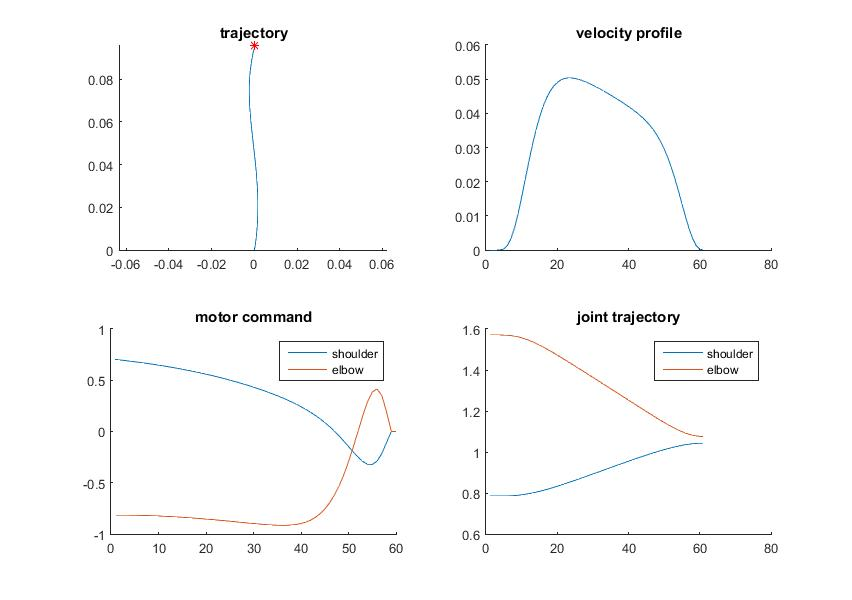
\includegraphics[width=\textwidth]{up8} 
	\caption{simulation result with high viscosity value}
	\label{fig:0.8}
\end{figure}
\begin{figure}[h]
	\centering
	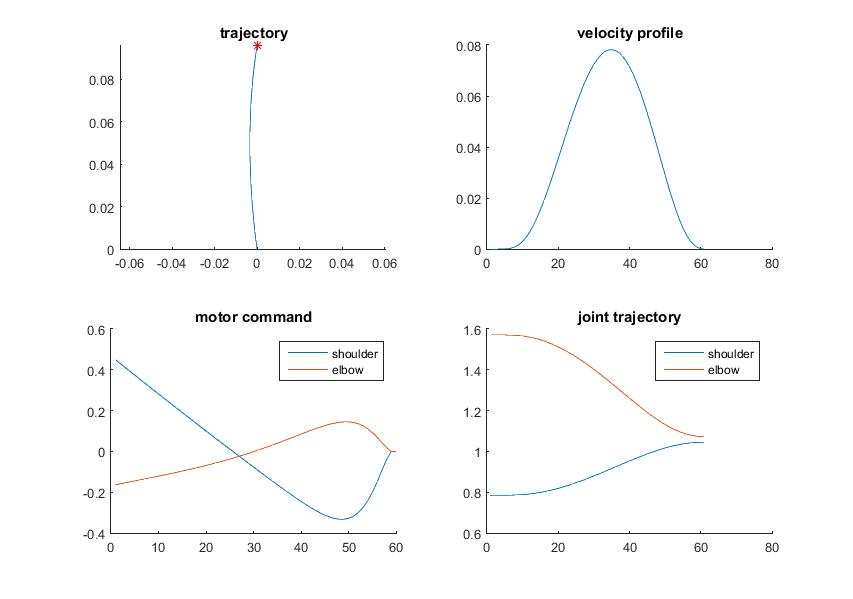
\includegraphics[width=\textwidth]{up0}
	\caption{simulation result with zero viscosity value}
	\label{fig 0.0}
\end{figure}
\end{singlespace}


% In case your dissertation has multiple volumes.
% \addvolumecontents{thesis_part2}
% \addvolumecontents{thesis_part3}
% \addvolumecontents[lof]{thesis_part2}

\end{document}
